% don't remove the following lines, and edit the definition of \main if needed
\documentclass[../report.tex]{subfiles}
\providecommand{\main}{..}
\IfEq{\jobname}{\currfilebase}{\AtEndDocument{\biblio}}{}
% until here
% this is a macro so you can make comments. See example below.
%\newcommand{\ew}{electro-weak\xspace}
\newcommand{\ew}{electroweak\xspace}
\newcommand{\met}{E_\textrm{T}^\textrm{miss}}
\newcommand{\epem}{e^{+}e^{-}}
\newcommand{\commentsinout}[1]{#1}
\newcommand{\KE}[1]{\commentsinout{\textbf{\color{brown} [KE: #1]}}} % Comments by K. Ellis
\newcommand{\FM}[1]{\commentsinout{\textbf{\color{orange} [FM: #1]}}} % Comments by F. Maltoni
\newcommand{\AN}[1]{\commentsinout{\textbf{\color{teal} [AN: #1]}}} % Comments by A. Nisati
\newcommand{\BH}[1]{\commentsinout{\textbf{\color{blue} [BH: #1]}}} % Comments by B. Heinemann

\newcommand{\ifb}{fb$^{-1}$}
\newcommand{\iab}{ab$^{-1}$}
\newcommand{\sintheta}{\sin^2\theta_W}
\newcommand{\etmiss}{E_\textrm{T}^\textrm{miss}}
\newcommand{\BR}{BR}
\newcommand{\BRinv}{BR$_{\textrm{inv}}$}
\newcommand{\BRunt}{BR$_{\textrm{unt}}$}

%\newcommand{\FCChh}{FCC-hh\xspace}
%\newcommand{\FCCee}{FCC-ee\xspace}
%\newcommand{\FCC}{FCC\xspace}
%\newcommand{\FCChhLowE}{FCC-hh, low energy\xspace}
%\newcommand{\FCCeh}{FCC-eh\xspace}
%\newcommand{\CLIC}{CLIC\xspace}
%\newcommand{\CEPC}{CEPC\xspace}
%\newcommand{\ILC}{ILC\xspace}
%\newcommand{\CLICThreeHundredEighty}{CLIC$_{380}$\xspace}
%\newcommand{\CLICThreeThousand}{CLIC$_{3000}$\xspace}
%\newcommand{\CLICfifteen}{CLIC$_{1500}$\xspace}
%\newcommand{\ILCTwoHundredFifty}{ILC$_{250}$\xspace}
%\newcommand{\ILCFiveHundred}{ILC$_{500}$\xspace}
%\newcommand{\ILCOneThousand}{ILC$_{1000}$\xspace}
%\newcommand{\HLLHC}{HL-LHC\xspace}
%\newcommand{\HELHC}{HE-LHC\xspace}
%\newcommand{\LHeC}{LHeC\xspace}

%\usepackage{hyperref}
%\usepackage{mathptmx}
%\usepackage{amsmath}
%\usepackage{xcolor}
\def\permille{\ensuremath{{}^\text{o}\mkern-5mu/\mkern-3mu_\text{oo}}}

\begin{document}
\linenumbers
% this is the extra information to be used for the general sections.
\chapter{Electroweak Physics}
\label{chap:ew}
In this chapter the status of the \ew physics programme and its future prospects are discussed. Particular emphasis is given to the exploration of the Higgs boson at the future colliders discussed in Chapter~\ref{chap:acc}.
%\BH{Need to add references to submissions}

\section{Introduction}
\label{sec:ewkintro}
The \ew sector of the Standard Model (SM) of particle physics is extraordinarily rich, and its theoretical elucidation and experimental exploration over the past 80 years is among the most outstanding scientific achievements of humankind. Components of that achievement are the invention of quantum electrodynamics (QED)~\cite{Dirac:1927dy}, the discovery of the weak interaction\cite{Fermi:1934hr,Sudarshan:1958vf,Feynman:1958ty}, the unification of the weak and electromagnetic interactions in the late 1960s~\cite{Weinberg:1967tq,Salam:1968rm}, the discoveries of the $W$ and $Z$ bosons in the 1980s~\cite{Rubbia:1985pv}, and last but not least the discovery of the Higgs boson in 2012~\cite{Aad:2012tfa,Chatrchyan:2012xdj}. In the perturbative regime, QED has been tested with a precision of one part in $10^{12}$, an amazing achievement of both experiment and theory. For the \ew theory, many tests have been made at the per mille level at high-energy colliders and low-energy experiments, all confirming the SM predictions.

Despite this huge success, the \ew sector of the SM is puzzling. In particular, if new physics occurs at a higher mass scale, there is no explanation for why the Higgs boson mass should be at $\sim 125$~GeV, rather than at the much higher scale. 
Indeed, quantum corrections to the Higgs boson mass, $\Delta m_H$, due to e.g. the top quark, are much larger than the Higgs boson mass itself, and there is no explanation for this. The natural expectation is that $(\Delta m_H)^2 \sim \Lambda^2$ where $\Lambda$ is the energy scale of new physics (see Chapter~\ref{chap:th}). 

This issue is called the naturalness problem (see also Chapter~\ref{chap:th}). The naturalness problem can be quantified by the ratio of the experimentally measured Higgs mass to the quantum corrections to the Higgs mass, i.e.
\begin{equation}
    \epsilon \equiv \frac{m_H^2}{(\Delta m_H)^2}\,,
\end{equation}
where $\Delta m_H$ is the sum of all quantum corrections to the Higgs boson mass, and can be calculated in any model. In the SM, where there is no new physics below the Planck scale, the value is $\Delta m_H\sim 10^{19}$~GeV, corresponding to an extreme fine-tuning $\epsilon\sim 10^{-34}$. Values of the parameter $\epsilon \sim 1$ correspond to no fine-tuning. Note that in the literature, it is common to express the fine-tuning in terms of $\Delta$ where $\Delta=1/\epsilon$.

Depending on how the new physics couples to SM particles, new physics models can be classified as \textit{soft}, \textit{super-soft} and \textit{hyper-soft}~\cite{Contino:2017moj}. An example for a soft model is the Minimal Supersymmetric Model (MSSM) with high-scale mediation of the soft terms, for super-soft examples are Composite Higgs (CH) models and SUSY models with low-scale mediation \textbf{(add refs or point to BSM chapter for this?)}. For hyper-soft models Neutral Naturalness is a prime example (see Chapter~\ref{chap:bsm}). In all cases, the fine tuning can be related to the mass of a putative top quark partner, $m_T$, as shown in Table~\ref{tab:finetuning}. Measurements of the Higgs boson couplings can also be related to the fine tuning parameter $\epsilon$ as shown in Table~\ref{tab:finetuning}.
Furthermore, $\epsilon$ can be related to the oblique parameters~\cite{Peskin:1990zt,Peskin:1991sw,Altarelli:1991fk,Golden:1990ig, Barbieri:2004qk}, $O$, which are introduced to quantify possible modifications of the \ew precision observables due to new physics. Here, parameters $S$ and $T$ are the focus; $T$ measures the difference between the new physics contributions of neutral and charged current processes at low energies and $S$ describes new physics contributions to neutral current processes at different energy scales.

\begin{table}[htbp]
    \centering
     \caption{Constraints on the fine tuning parameter, $\epsilon$, as determined via direct searches and via precision measurements of Higgs boson couplings and oblique parameters. For direct searches $m_T$ is the mass of the top quark partner, and $y_t$ and $\lambda_h$ are coupling parameters which are both assumed to be $\sim 1$ in natural theories. %The oblique parameter is related to the coupling, $g_*$, and mass, $m_*$, of new physics via $\delta \hat{O}\propto g_*^2/m_*^2\times N$, where $N$ is the number of degrees of freedom. 
     For the direct searches and the oblique parameters, the mass value used for interpretation as $\epsilon$ is $m_T=1$~TeV, motivated by current limits on top partners\cite{atlasstop,cmsstop,atlasvtop,cmsvtop}. CH stands for "composite Higgs" and SUSY for "supersymmetry".
     %\BH{Asked Riccardo if it is really $\pi^2$ in the 2nd equation. And, other things. Waiting for answer.}
    \label{tab:finetuning}}
    \begin{tabular}{l|l|r}
    \hline
    Method & Dependence & Current Constraint \\\hline\hline
         Direct searches: soft models  & $\Delta m_H^2 \sim m_T^2$ & $\epsilon\lesssim 1\%$ \\
        Direct searches: super-soft models & $\Delta m_H^2 \sim 3y_t^2/(4\pi^2)
    m_T^2$  & $\epsilon\lesssim 10\%$\\
        Direct searches: hyper-soft models & $\Delta m_H^2 \sim 3\lambda_h/(16\pi^2) m_T^2$  & $\epsilon \lesssim 100\%$\\\hline
         Higgs couplings & $m_H^2/\Delta m_H^2\sim \delta g_h/g_h$ & $\epsilon \lesssim 10\%$\\
         Oblique parameters (CH models)& $
         m_H^2/\Delta m_H^2 \sim 
         \delta O\times 3$ 
          & $\epsilon \lesssim 30\%$ \\
          Oblique parameters (SUSY models)& $
         m_H^2/\Delta m_H^2 \sim 
         \delta O\times 10^{3}$ 
          & n.a. \\
          \hline
    \end{tabular}
\end{table}
Based on these arguments, it is clear that measurements of Higgs boson couplings at the \% level or better test new physics models at or beyond the current constraints from direct searches. The same is true when the oblique parameters are measured to better than $\sim 3\times 10^{-3}$. Future direct searches at the FCC-hh or a muon collider are expected to improve the sensitivity to the top quark partner to 10~TeV, and thus be sensitive to values of $10^{-3}-10^{-5}$ (see Chapter~\ref{chap:bsm}). 

\subsection{Higgs studies at hadron colliders}
Figure~\ref{fig:Higgs_XS_7-100TeV_HH} shows the cross
sections for the production of Higgs bosons from LHC energies to the energy of \FCChh. 
So far at the LHC, about 8 million Higgs bosons have been produced and the data sample will further increase by a factor of 20 at the conclusion of \HLLHC.
\begin{figure}[t]
\centering
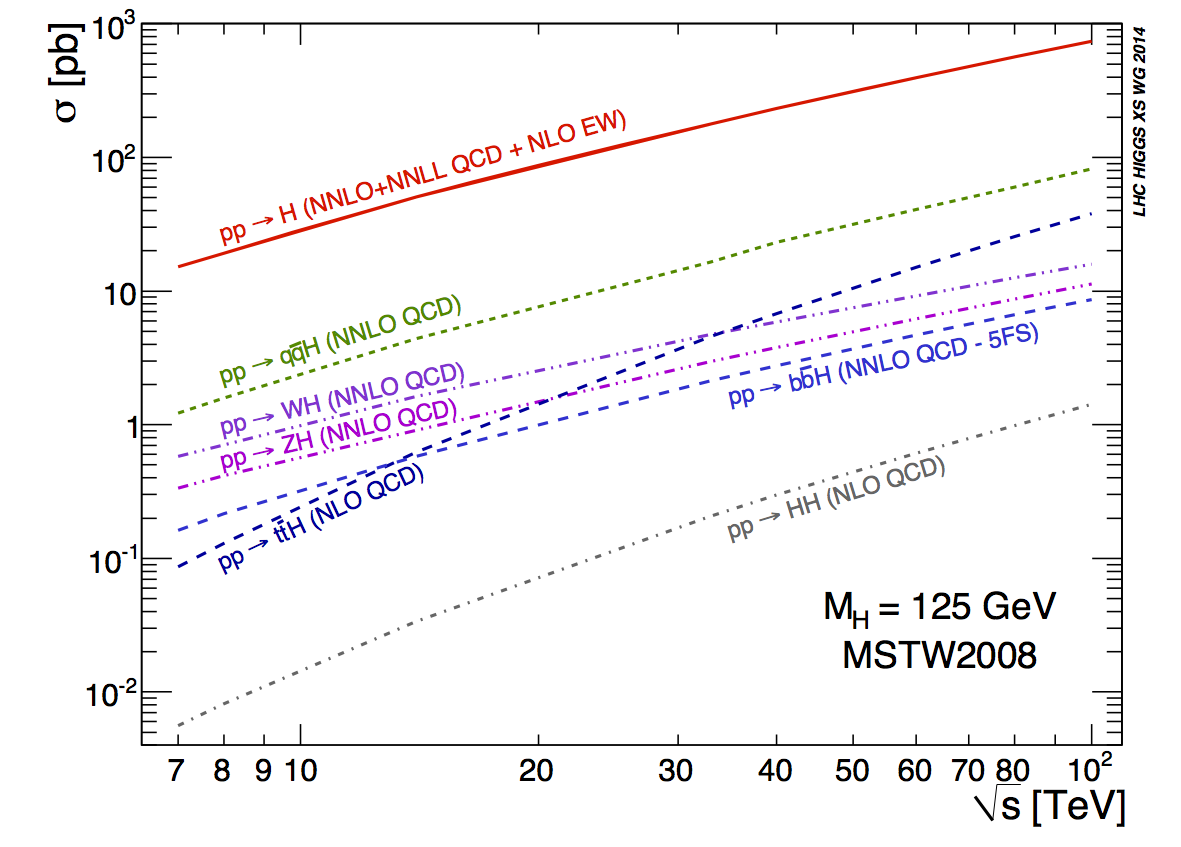
\includegraphics[width=.8\linewidth]{\main/ewksection/img/Higgs_XS_7-100TeV_HH.png}
\caption{\label{fig:Higgs_XS_7-100TeV_HH}
Higgs production cross sections in hadronic collisions.}
\end{figure}
The coupling parameters themselves cannot be extracted at hadron colliders without further assumptions which depend on the new physics model. 
In particular, to resolve a multiplicative ambiguity in inferring couplings from measured cross section times decay branching ratio ($\sigma(H) \times {\rm BR}$) values, it is usually assumed either that there are no new light states that the Higgs boson can decay to (i.e. the Higgs width is fully determined by the couplings to the SM particles), or that the coupling to the gauge bosons can not be larger than the SM value.  This latter assumption is valid for the vast majority of beyond the standard models, and is made for results and projections presented here. 

Figure~\ref{fig:higgsnow} presents a selection of current Higgs coupling measurements~\cite{atlashcomb2,cmshcomb2} and the precision projected for HL-LHC~\cite{Cepeda:2019klc}, with the constraint $|\kappa_V|\leq 1$. Here, $\kappa_i$ is a parameter which specifies by how much the coupling of the Higgs boson to a given particle $i$ deviates from the SM expectation, see Sec.~\ref{sec:higgsfuture} for more details. The current uncertainties are typically 10-20\% for the bosons and 3rd generation fermions. For the muon coupling modifier the uncertainty is about 100\%, and the upper limits on new invisible or undetected particles are 20-30\%. With the \HLLHC, the precision will be improved by about a factor of 5-10 on all observables. Figure~\ref{fig:higgsnow} also shows the composition of the expected \HLLHC uncertainties in a $\kappa$-fit where the width is assumed to be fully determined by the couplings to the SM particles. The only channels which are expected to be limited by data statistics are the rare decays to muons and $Z\gamma$. In all other cases, the experimental systematic uncertainties are similar to the statistical uncertainties, but the dominant source of uncertainty arises from theory. Here, it is already assumed that the theory uncertainties can be reduced by a factor of two compared to the current uncertainties which is challenging to achieve. For both hadron and lepton colliders, a further reduction of theory uncertainties is pivotal to fully capitalise on the experimental data. Section~\ref{sec:ewktheory} discusses the status and prospects for theory uncertainties.

\begin{figure}[htbp]
    \centering
    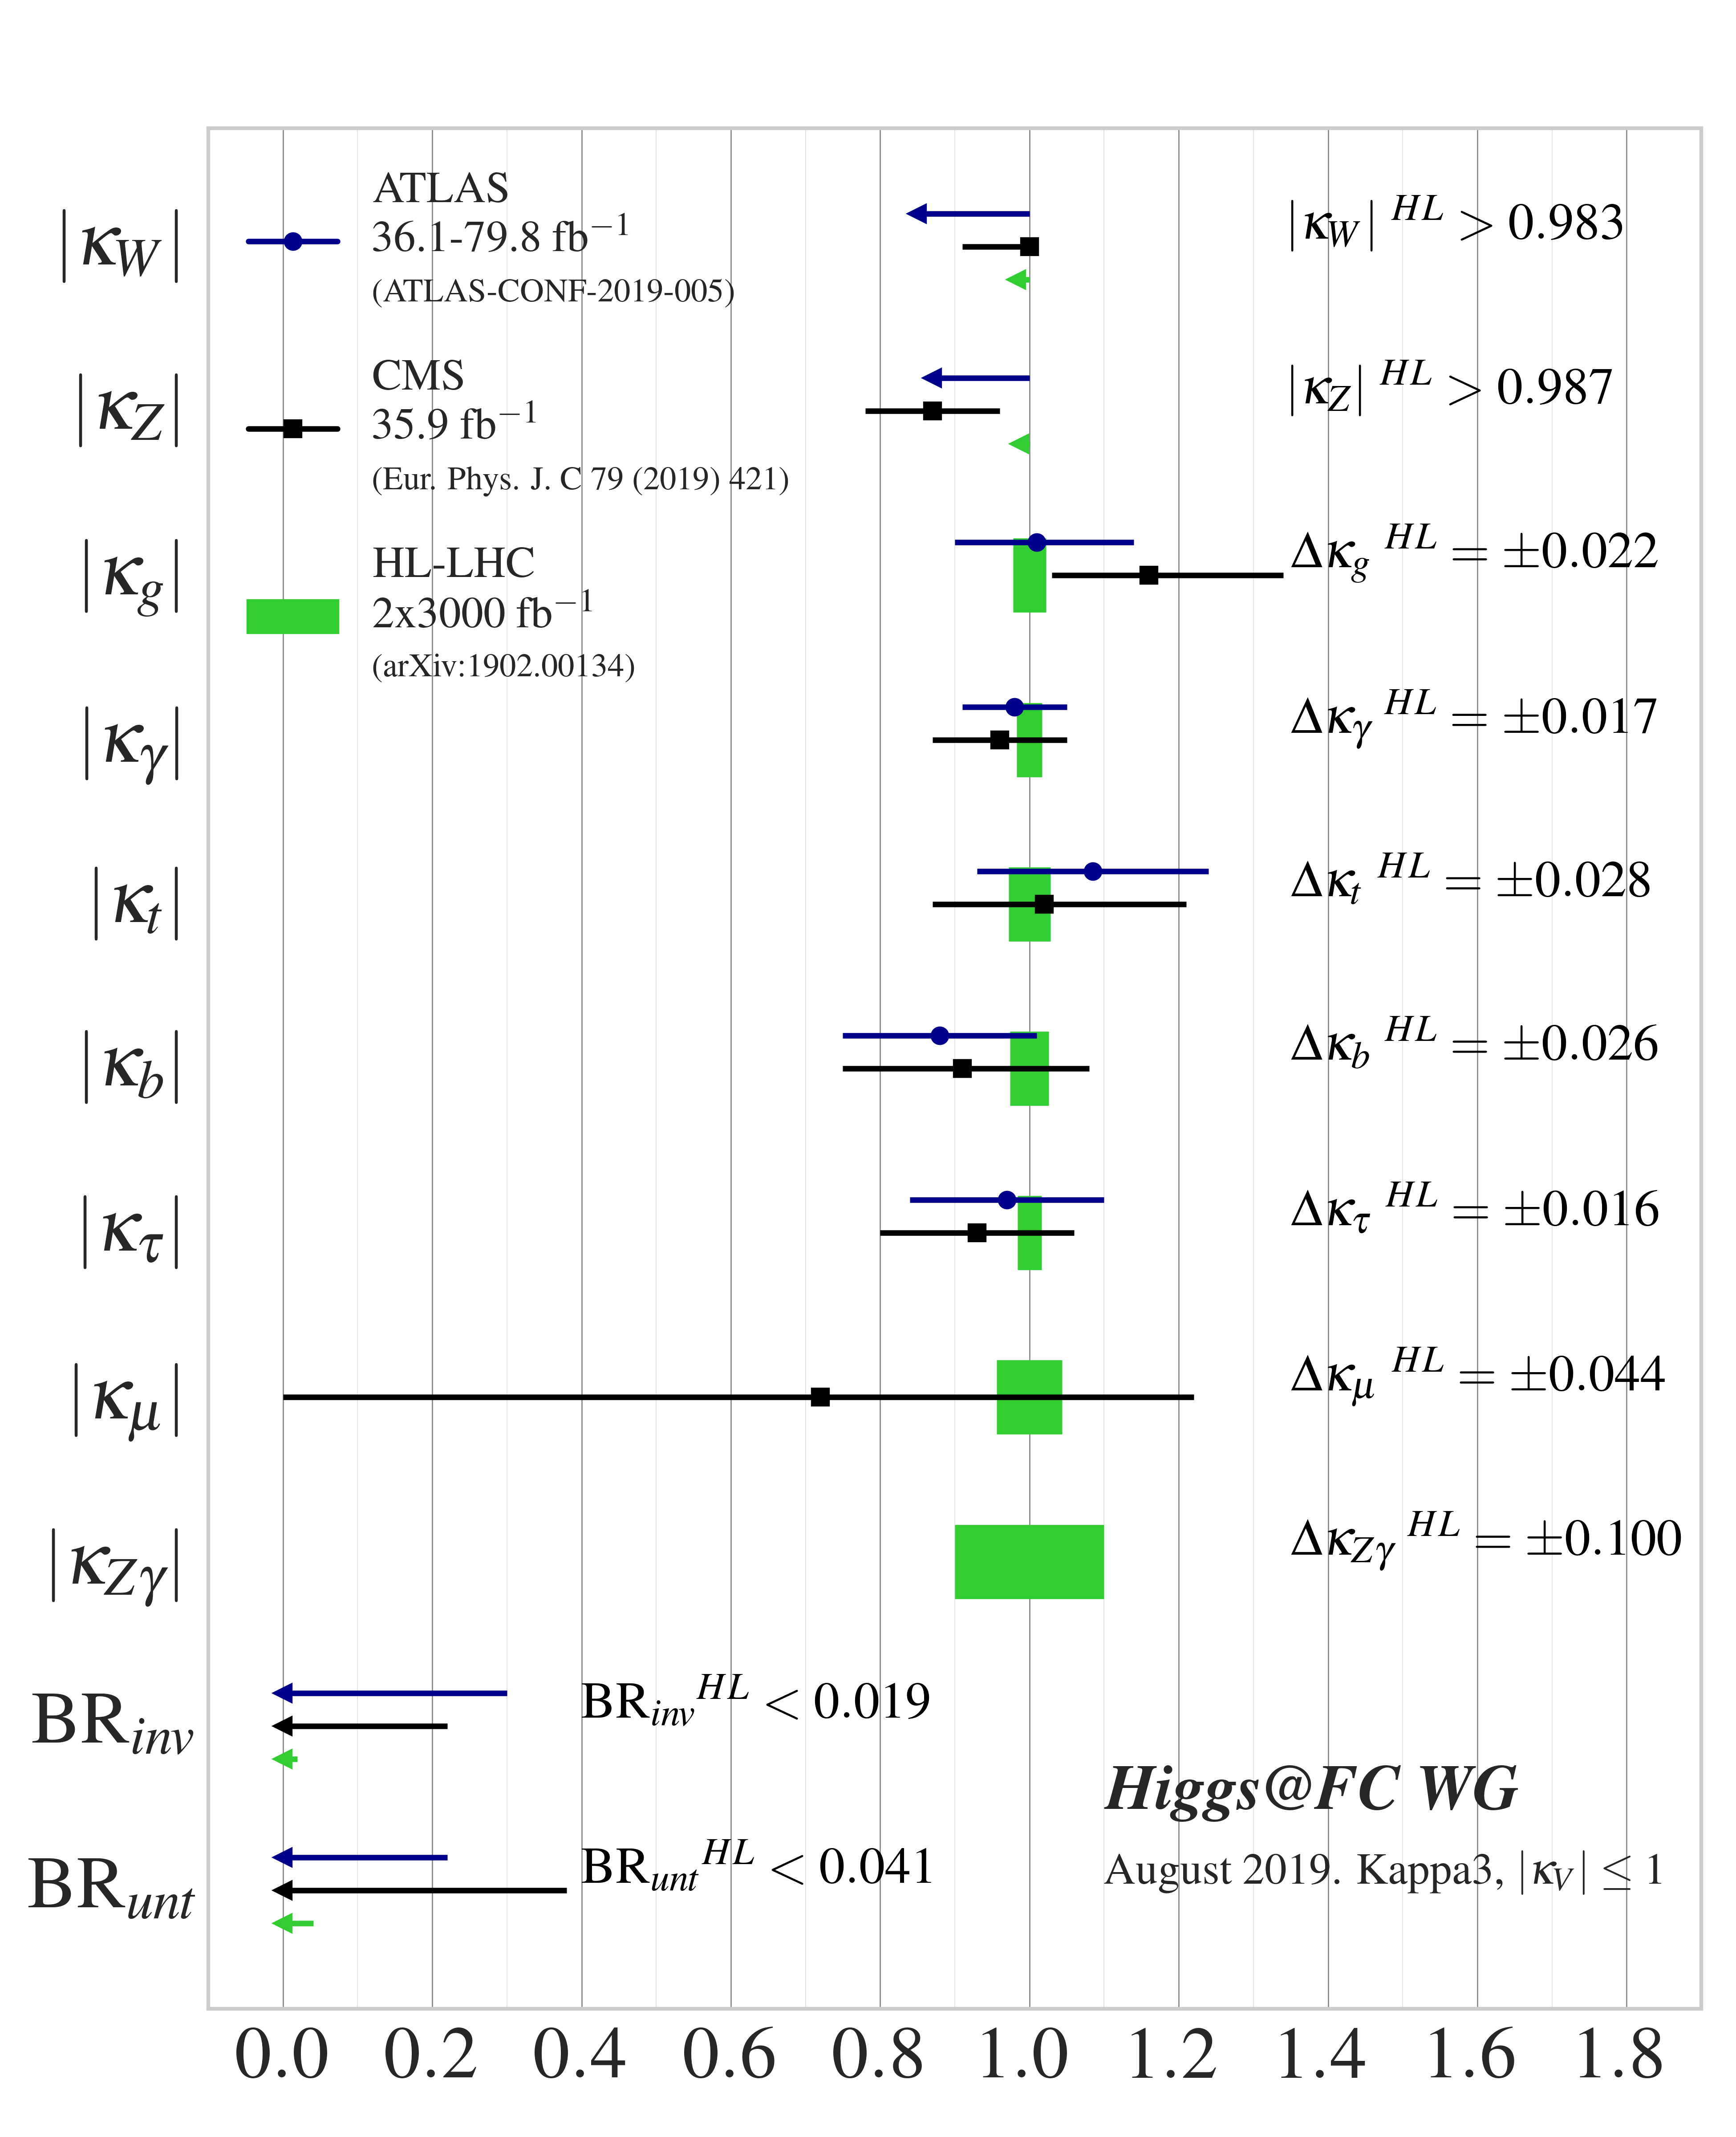
\includegraphics[width=.44\linewidth]{\main/ewksection/img/Figure1ComparisonRun2HL.png}
    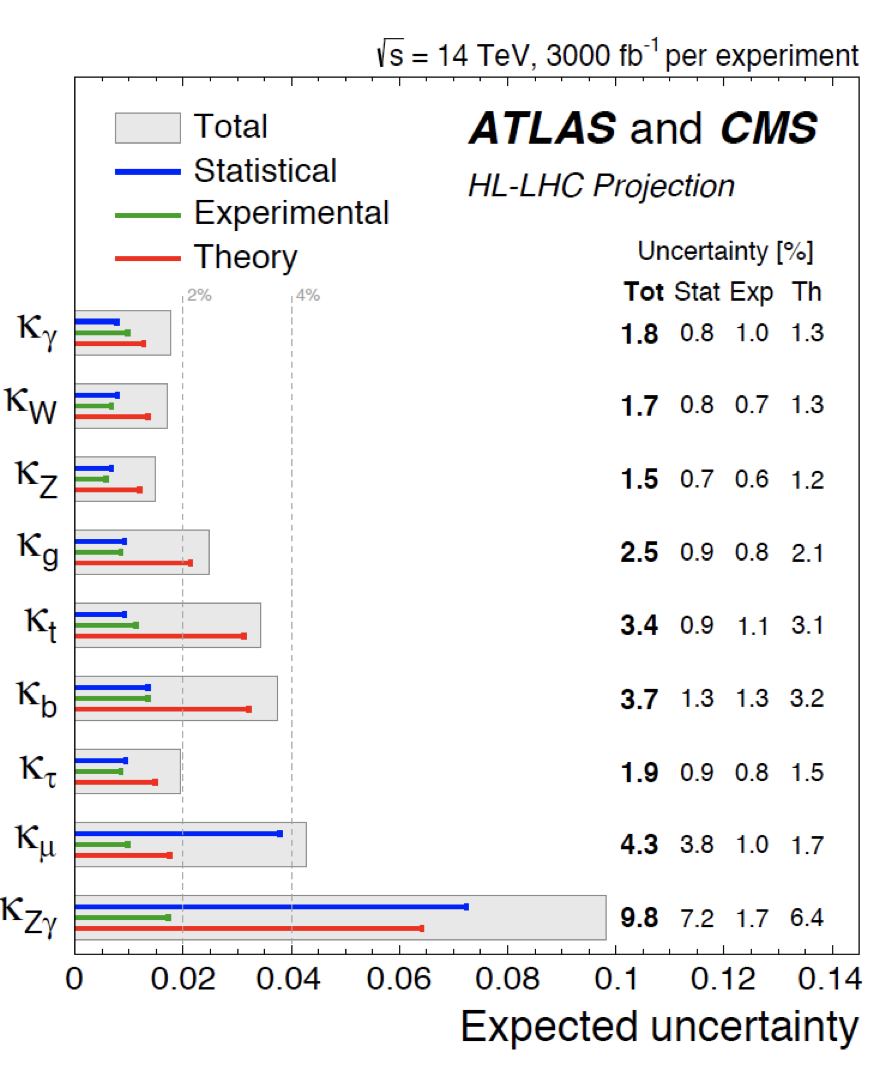
\includegraphics[width=.45\linewidth]{\main/ewksection/img/kappa_hllhc.png}
    \caption{Left: Relative precision on Higgs coupling modifiers, $\kappa$, determined by ATLAS and CMS with the LHC data at present, and as expected for \HLLHC with the constraint $\kappa_V\leq 1$. Also shown are the constraints on invisible and undetected decay branching ratios, \BRinv and \BRunt. Right:  Expected uncertainty on Higgs coupling parameters at \HLLHC, showing separately the statistical, experimental and theoretical uncertainties. Here, it was assumed that the branching ratios (BR's) to untagged and invisible decays are zero.
    \label{fig:higgsnow}}
\end{figure}

\subsection{Higgs studies at $e^+ e^-$ colliders}
The Higgs production processes in unpolarised $e^+e^-$ collisions are shown in Fig.~\ref{fig:xsec_vs_cme}.
\begin{figure}[!ht]
\centering
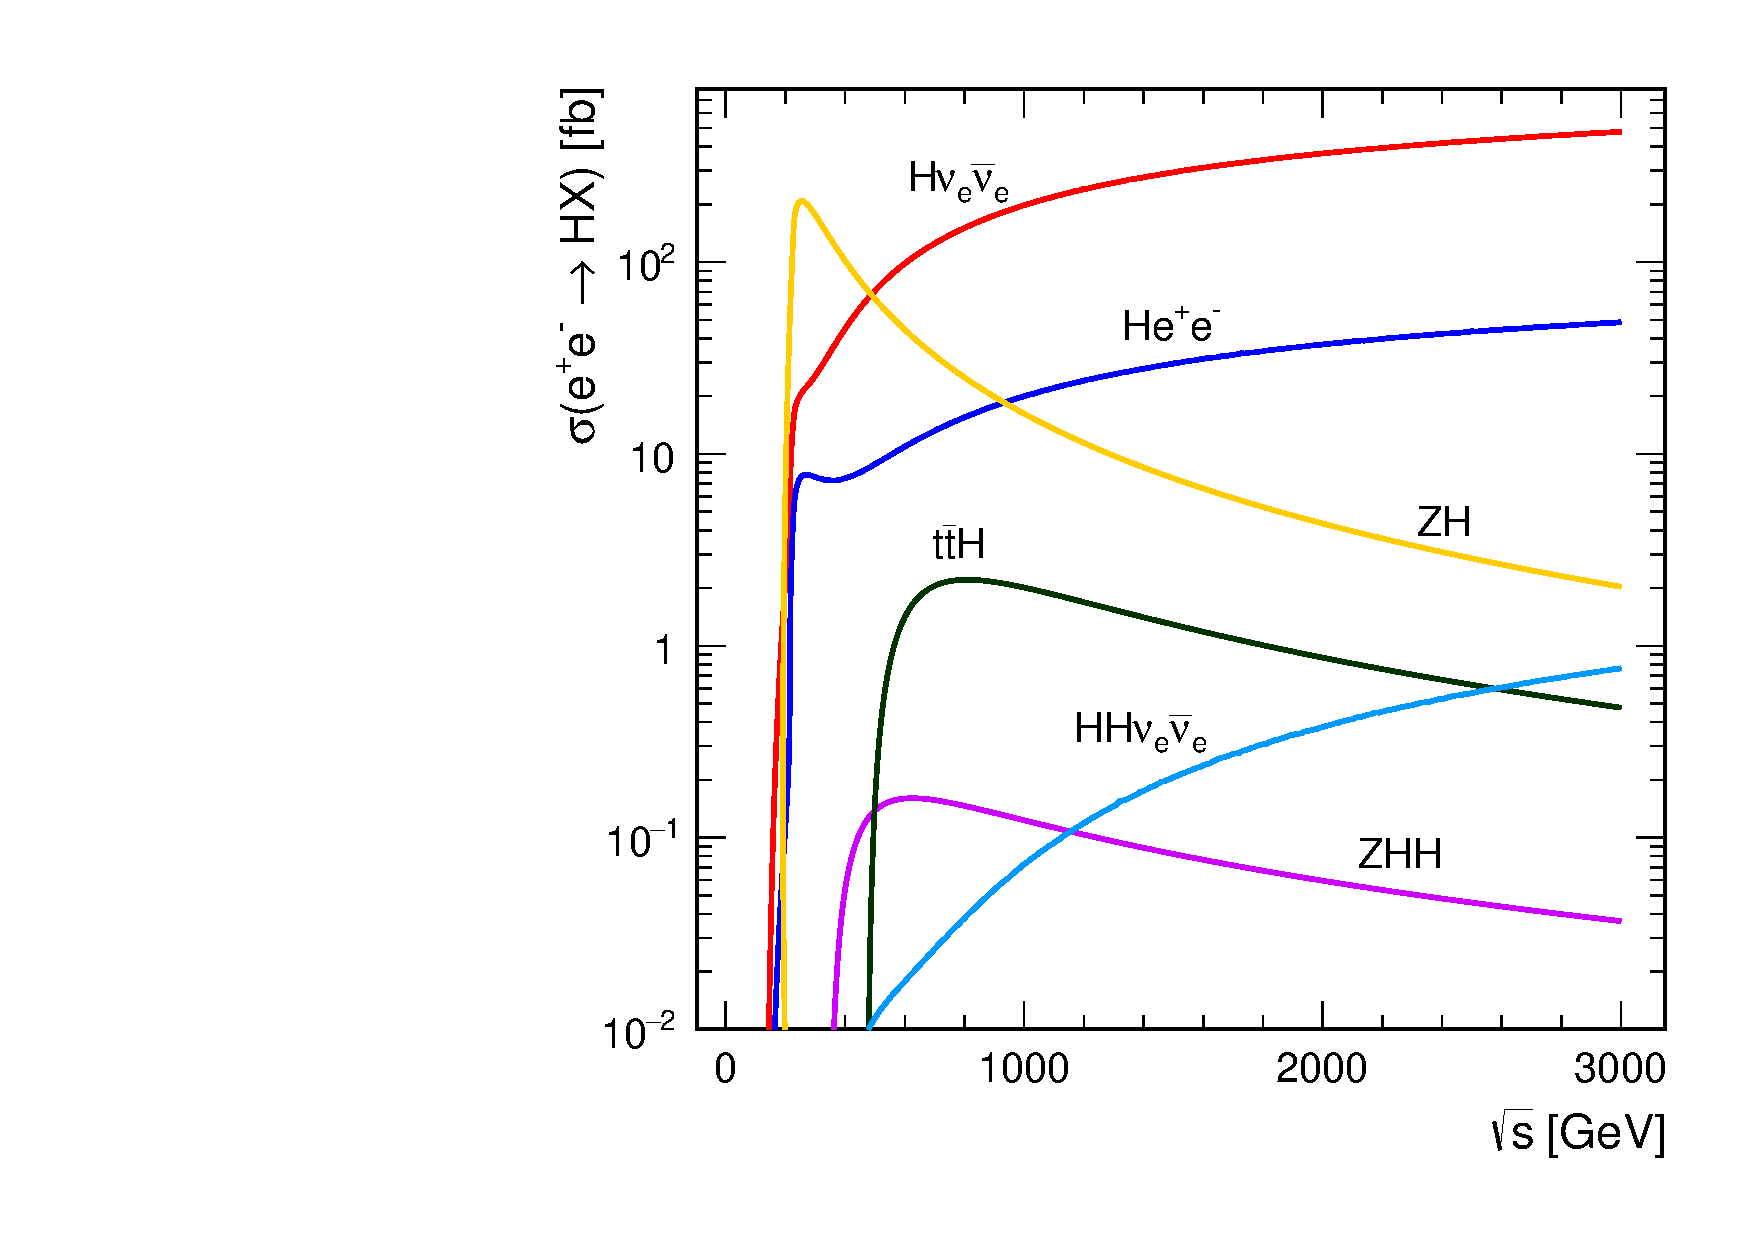
\includegraphics[width=.6\linewidth]{\main/ewksection/img/xsec_vs_cme.pdf}
\caption{\label{fig:xsec_vs_cme}
Higgs production cross sections in $e^+e^-$ collisions\cite{Abramowicz:2016zbo}. The cross section of different production processes for single and double Higgs production are shown as function of $\sqrt{s}$.}
\end{figure}
Importantly the total $ZH$ cross section can be measured  independent of the Higgs boson decay, using a missing mass technique. From this measurement the coupling $g_{ZZH}$ can be derived. Consequently, at an $e^+ e^-$ collider, the Higgs total width ($\Gamma_H$) can be determined
from $\Gamma(H\to ZZ^*)/BR(H \to ZZ^*)$	thus removing the ambiguity on the Higgs width that afflicts all measurements at hadronic machines.
Polarisation is expected at the linear machines $e^+e^-$ machines, e.g.
$|P(e^{-})|=0.8,|P(e^{+})|=0.3$ is projected to be achievable for the \ILC.
As shown in Table~\ref{tab:higgs:polarisation}, with the appropriate polarisation this can enhance the Higgs boson production cross section.
In addition, because the importance of different subprocesses can be tuned by changing the polarisation, it plays an important role in effective operator fits.
Thus, the presence of polarisation can sharpen these analyses, and helps compensate for the lower luminosities at linear machines.
\begin{table}[tb]
\caption{The dependence of the event rates for the $s$-channel
$\epem\to Z H$ process and the pure $t$-channel
$\epem\to H \nu_e \nu_e$ and $\epem\to H\epem$ processes for several
example beam polarisations~\cite{Abramowicz:2016zbo}.
\label{tab:higgs:polarisation}}
\begin{center}
  \begin{tabular}{cccc}
    Polarisation                              & Scaling factor                 &&       \\
\hline
    $P(e^{-}):P(e^{+})$                  &
    $\epem \!\to ZH$ &
    $\epem \to H\nu_e \bar{\nu}_e$ &
    $\epem \to H\epem$ \\
    unpolarised                                  & 1.00                & 1.00        &   1.00        \\
    $-80\,\%\,:\phantom{+3}\,0\,\%$   & 1.12                & 1.80        &    1.12             \\
    $-80\,\%\,:\,+30\,\%$                    & 1.40                & 2.34        &    1.17           \\
    $-80\,\%\,:\,-30\,\%$                    & 0.83                & 1.26        &    1.07           \\
    $+80\,\%\,:\phantom{+3}\,0\,\%$  & 0.88                & 0.20        &    0.88             \\
    $+80\,\%\,:\,+30\,\%$                    & 0.69                & 0.26        &    0.92           \\

    $+80\,\%\,:\,-30\,\%$                    & 1.08                & 0.14        &    0.84           \\
\hline
\end{tabular}
\end{center}
\end{table}


%\begin{figure}[!ht]
%\centering
%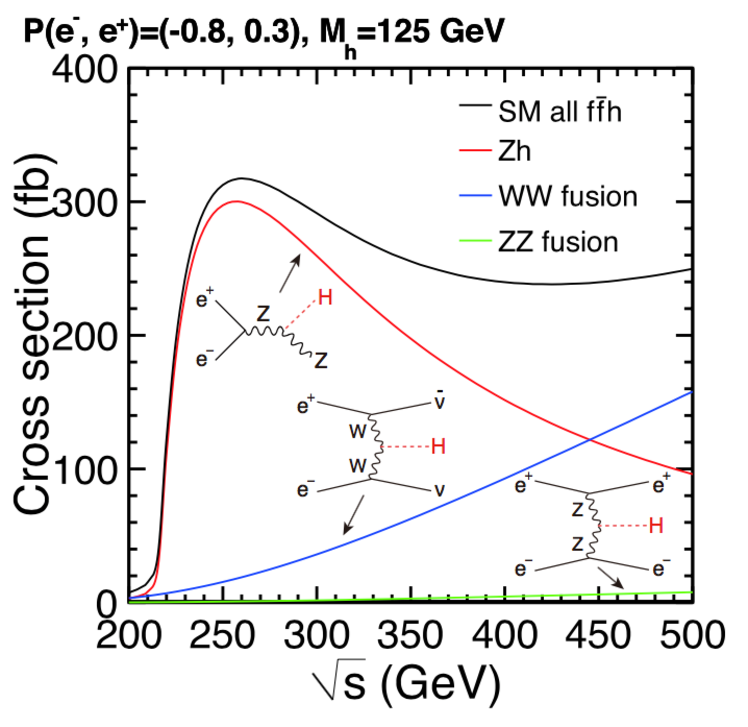
\includegraphics[width=.8\linewidth]{\main/ewksection/img/xsec_h_ILC_left.pdf}
%\caption{\label{fig:xsec_h_ILC_left}
%Higgs production cross sections in $e^+e^-$ collisions\cite{Fujii:2017vwa}
%for the polarization at ILC.}
%\end{figure}

\subsection{Electroweak Precision Observables}
Loop corrections to \ew precision observables (EWPO) provide a powerful test of the consistency of the SM. The relation between e.g. the  Fermi constant ($G_F$), Weinberg angle ($\sin^2\theta_W$), and the masses of the $Z$, $W$ and $H$ bosons ($m_Z$, $m_W$, $m_H$) and the top quark ($m_\textrm{top}$) is precisely predicted in the SM. Inconsistencies between these would indicate contributions from new physics.

These contributions are currently constrained primarily by the $Z$ pole measurements made at the LEP experiments and SLD~\cite{ALEPH:2010aa}, measurements of $WW$ production at LEP-2~\cite{LEP-2} and measurements of $W$-boson and top quark masses at the Tevatron~\cite{tevmw,tevmtop} and LHC~\cite{Aaboud:2017svj,Tokar:2019wny} experiments, and $m_H$ measurements at the LHC~\cite{Aaboud:2018wps, Sirunyan:2017exp}. The current constraints on the EWPO are shown in Fig.~\ref{fig:ewknow}. All measurements agree within the current precision.

Based on the \ew precision measurements, the 95\% CL upper limits on the oblique parameters~\cite{Peskin:1990zt} are $S<0.18$ and $T<0.26$~\cite{Tanabashi:2018oca}. Fig.~\ref{fig:ewknow} shows $T$ vs $S$ and illustrates how the various precision measurements on $\Gamma_Z$, $M_W$ and asymmetries contribute. 
 
\begin{figure}[h]
    \centering
    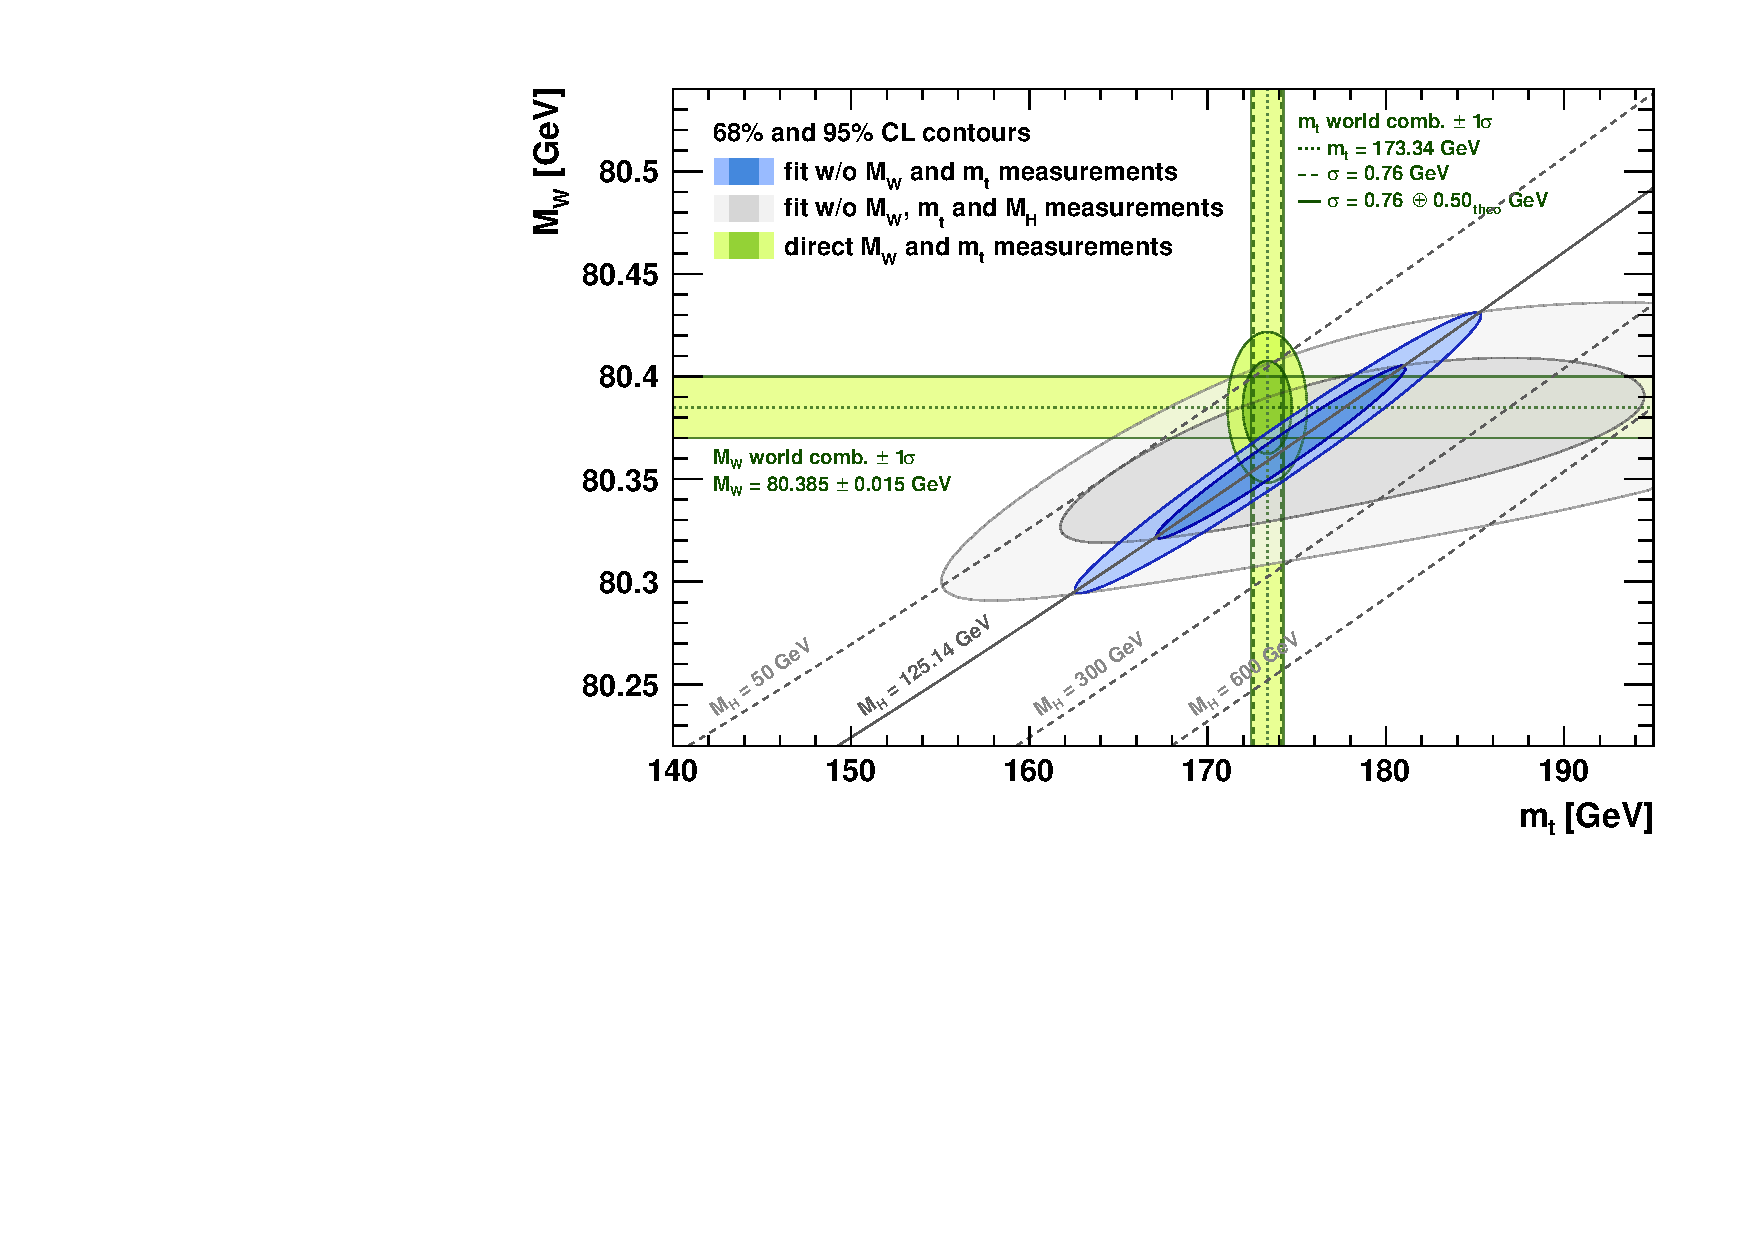
\includegraphics[width=.54\linewidth]{\main/ewksection/img/Scan2D_MWvsmt.pdf}
    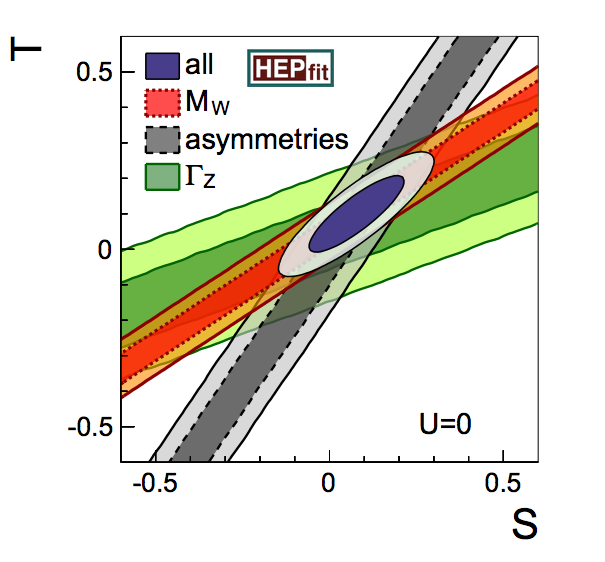
\includegraphics[width=.44\linewidth]{\main/ewksection/img/ElectroweakPhysics-front.png}
\caption{
Left: Constraints on the $W$-boson and top-quark mass from direct measurements and indirect constraints~\cite{Baak:2014ora}. 
Right: Constraints on the oblique parameters $S$ and $T$ (fixing a third oblique parameter $U = 0$), 
together with the individual constraints from $M_W$, the
asymmetry parameters $\sin^2\theta^{lept}_{eff}$, $P_{pol}^{\tau}$
and the forward-backward asymmetries $A_{FB}^{f}$ with $f = \ell, c, b$, and $\Gamma_Z$. The dark (light) region corresponds to 68\% (95\%) probability~\cite{deBlas:2016ojx}.
    \label{fig:ewknow}}
\end{figure}

Measurements of diboson production are also sensitive to the \ew symmetry breaking mechanism as they depend on the trilinear gauge couplings of the bosons to each other. In addition, some processes, such as  $pp\to W^\pm W^\pm +2$~jets,  are  also sensitive to the quartic coupling of the $W$ bosons and to the coupling of the Higgs boson to $W$ bosons. 

In addition, at future $e^+e^-$ colliders, a campaign of \ew  measurements at the $Z$-pole and at the $WW$ threshold is also foreseen.

\subsection{The Higgs potential}
A very important aspect of the \ew physics programme is the measurement of the trilinear and quartic couplings of the Higgs boson to itself. These couplings are directly related to the shape of the Higgs potential, 
\begin{equation}\label{eq:SMpotential}
V(h)= \frac{1}{2} m_H^2 h^2 + \lambda_3 v h^3 + \frac{1}{4}\lambda_4 h^4,\qquad \textrm{with}\quad \lambda_3^{\rm SM}= \lambda_4^{\rm SM}= \frac{m_H^2}{2 v^2},
\end{equation}
where $v=1/\sqrt{\sqrt{2}G_F}\approx 246$\,GeV is the vacuum expectation value of the Higgs field, and $m_H\approx 125$~GeV.

The shape of the Higgs potential can have important consequences for our Universe as it determines how the early Universe went through a phase transition. In the early universe, the \ew phase transition is determined by the scalar potential at finite temperature, whereas collider measurements probe the potential at
zero temperature.
At a temperature of about 100~GeV it went from a symmetric state into a state with a broken \ew symmetry. For the SM Higgs potential, this phase transition is a crossover, but alterations to the potential could result in this phase transition having been first order. 
If the phase transition is strongly first order ($\lambda_3$ is modified by $O(1)$), and there is a new mechanism for CP violation, two of Sakharov conditions necessary (but not sufficient) for an explanation of matter and anti-matter asymmetry of the Universe are fulfilled.
Gravitational waves stemming from that phase transition could be discovered by the Laser Interferometer Space Antenna (LISA)~\cite{Caprini:2015zlo}.  

The parameters $\lambda_3$ and $\lambda_4$ can be measured in processes where two or three Higgs bosons are produced, and via loop-contributions in single Higgs production processes. At present, the LHC data are not sensitive but with \HLLHC it is expected that the trilinear Higgs self-coupling can be determined with a precision of about 50\%~\cite{Cepeda:2019klc}. 

\subsection{The Higgs boson and new particles}
The Higgs boson is also potentially a window of discovery for new particles, in particular of those having a mass $m<m_H/2$, into which the Higgs boson can decay. Thus even particles that do not interact with any SM particles except the Higgs boson, can be discovered using this new channel. These might be invisible, such as e.g. dark matter candidates, and result in the experimental signature of $\met$, or may be in principle detectable. These can be searched for via global coupling analyses as well as through targeted analyses, see Chapter~\ref{chap:bsm}. The present constraints and the anticipated \HLLHC constraints for global analyses are presented in Fig.~\ref{fig:higgsnow}. With \HLLHC (using the constraint $|\kappa_V| \leq 1$) such invisible and untagged decays will be probed at the few \% level. However, without the $|\kappa_V|\leq 1$ constraint, the BR to untagged decays is essentially unconstrained at the LHC through the inclusive coupling analysis, and only direct searches for anomalous decays provide sensitivity, as discussed in Chapter~\ref{chap:bsm}. 

\section{Future prospects}
%\textbf{this should be about 70\% of the text. I suggest we have three subsections}
\subsection{Electroweak precision measurements}
The precision of many observables related to the \ew bosons can be improved at future experiments. In particular, the proposed $e^+e^-$ colliders will be able to advance the precision measurements of the $W$- and $Z$-boson properties significantly. Figure~\ref{fig:ewkprogramme} shows the number of $Z$ and $W$ bosons that will be recorded at the various lepton colliders. For the circular colliders there are dedicated runs planned on the $Z$ pole and at the $WW$ threshold to make precise measurements of $Z$ boson properties and the $W$-boson mass, respectively. Since for circular colliders the luminosity increases with decreasing $\sqrt{s}$ more than $10^{11}$ $Z$ bosons will be recorded per year for CEPC and \FCCee. For the linear colliders, \ILC and \CLIC, the default plan foresees no running at energies below 250 and 380~GeV, respectively, but such an option could be added. Within a few years a sample of a few $10^9$ $Z$ bosons could be recorded~\cite{gigazilc,gigazclic}. In addition, a significant improvement for some of the $Z$ boson properties can also be achieved using $Z$ bosons during the default running at higher energies; those numbers are also shown in Fig.~\ref{fig:ewkprogramme} for \ILC and \CLIC.  

\begin{figure}[htbp]
    \centering
    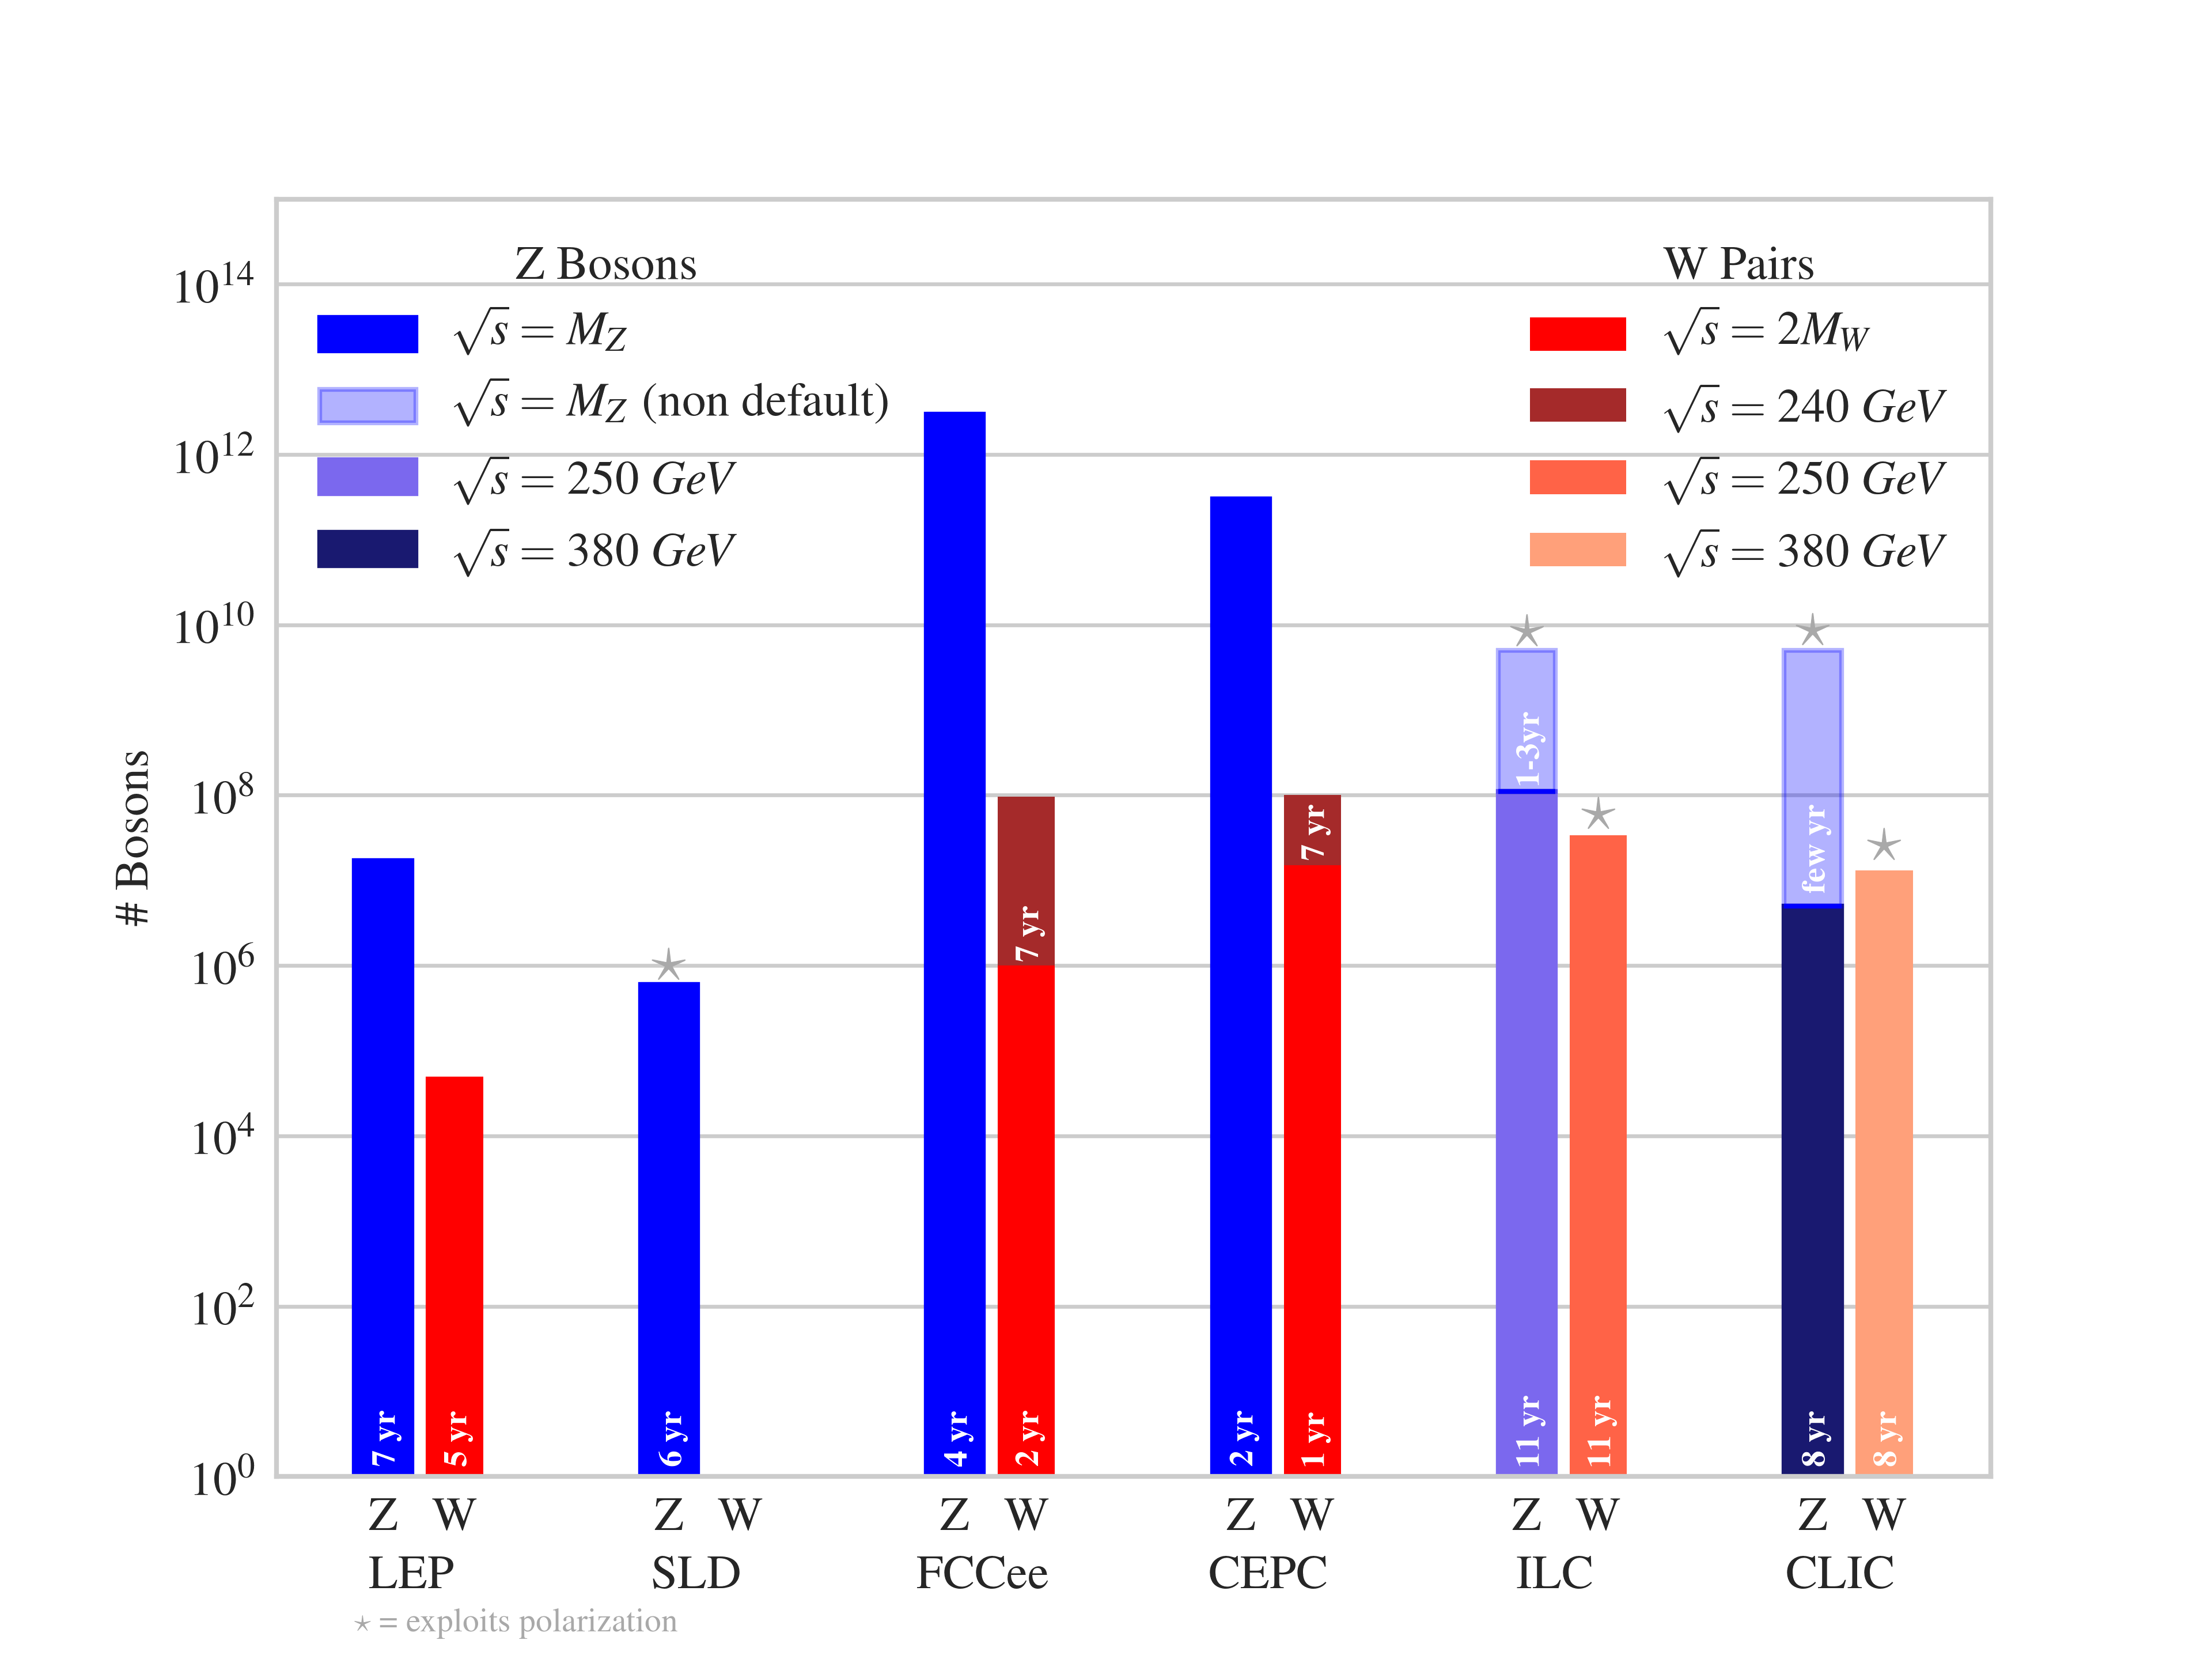
\includegraphics[width=.75\linewidth]{\main/ewksection/img/bosoncount}
    \caption{Number of $Z$ bosons and $W^+W^-$ boson pairs at past and future $e^+e^-$ colliders. The numbers are summed over experiments (four for LEP, two for \FCCee and \CEPC and one for the other colliders). For LEP the number of $W$ pairs shown includes all energies $\sqrt{s}\gtrsim 2M_W$.
    \label{fig:ewkprogramme}}
\end{figure}

Figure~\ref{fig:ewkpar} shows a selection of important EWPO, comparing the current precision to the future prospects at various future colliders. It is seen that all colliders will result in a significant improvement with respect to the current precision. For instance, the width of the $Z$ boson will be improved by about a factor of 20 by the \FCCee, and the decay rates and asymmetries (which are important for constraining the left- and right-handed couplings of the fermions) are typically improved by a factor of 10 or more. For the linear colliders, even with the running at $\sqrt{s}=250-380$~GeV a significant improvement compared to the current precision is achieved on most observables but dedicated running can add an additional large factor, close to the precision achieved by the circular machines, in many observables~\footnote{The reason for this similarity is that all measurements are expected to be dominated by systematic uncertainties; if the circular colliders can use the higher statistics to constrain these effectively the situation could change.}. 

\begin{figure}[htbp]
    \centering
%    \includegraphics[width=.9\linewidth]{\main/ewksection/img/EWKSummary2}
%    \includegraphics[width=.9\linewidth]{\main/ewksection/img/EWKSummary19August.png}
    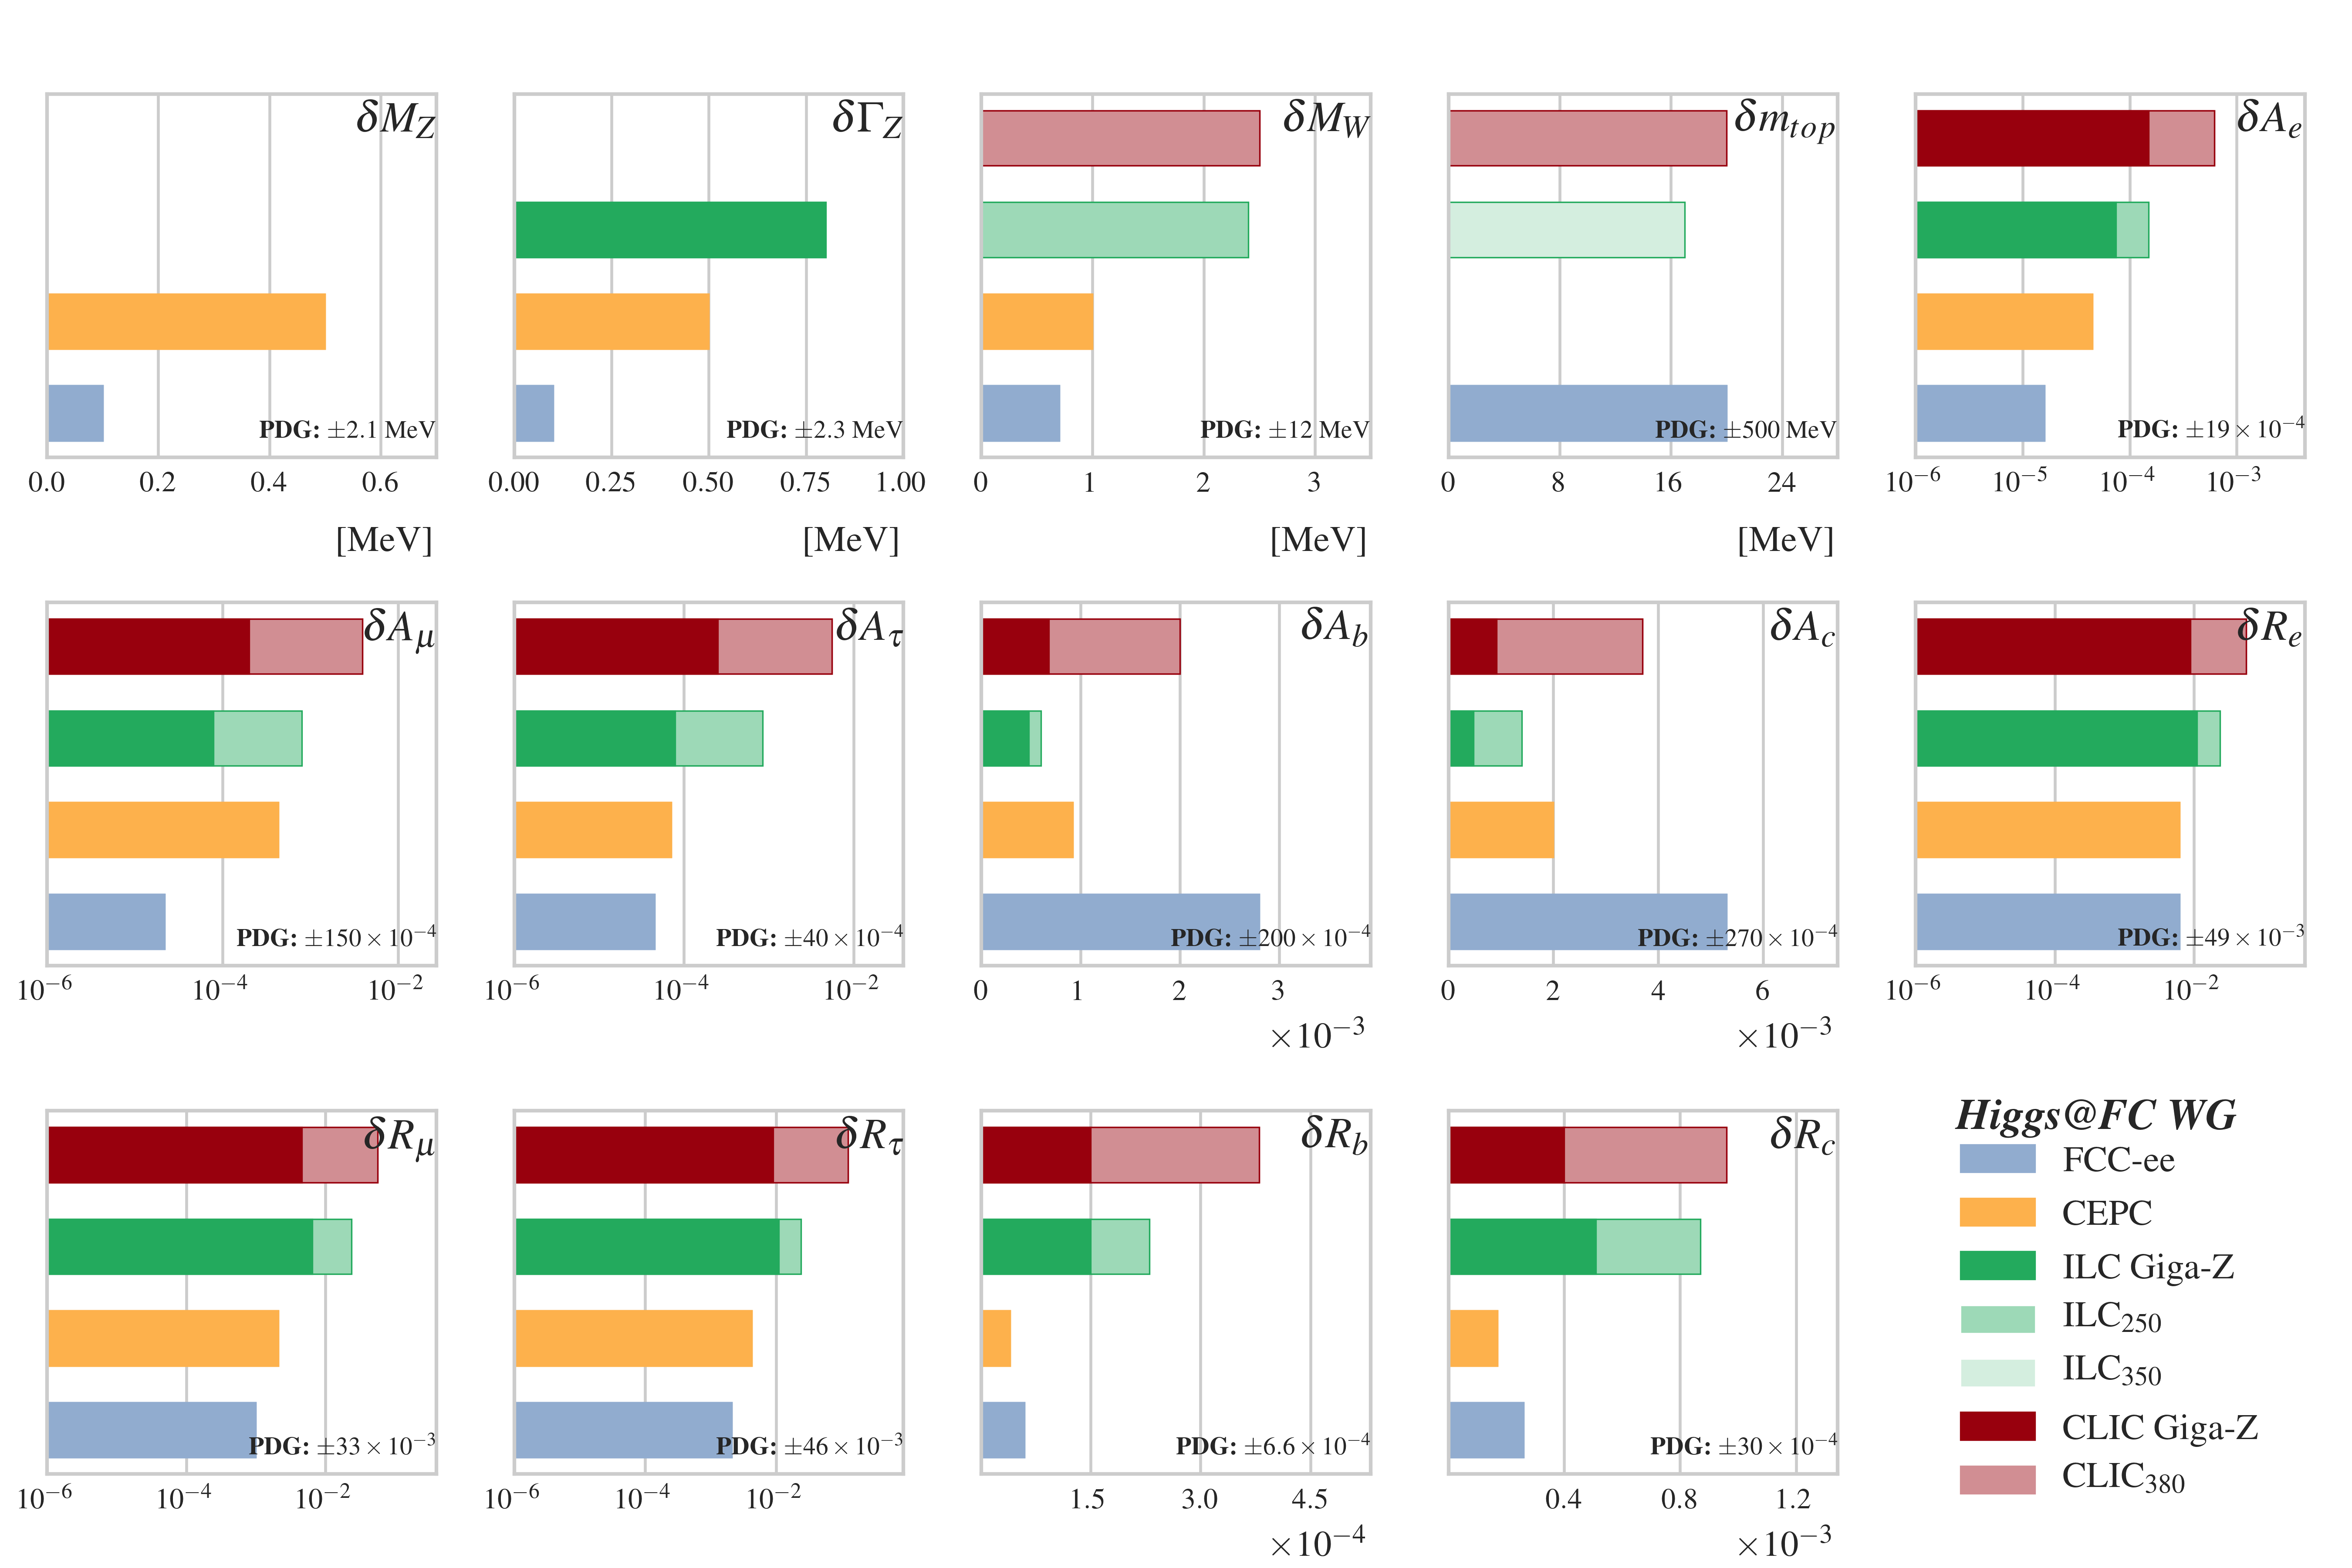
\includegraphics[width=.9\linewidth]{\main/ewksection/img/EWKSummary20August.png}
    \caption{Uncertainty on several observables related to the properties of the \ew bosons: the masses of the $Z$ and $W$ boson and the top quark, the $Z$ boson width, and for fermion $f$ the polarisation asymmetries ($A_f$) and ratios of decay rates relative to the total hadronic decay rate ($R_f$). The fermions considered are leptons and b- and c-quarks. For $A_b$ and $A_c$, \FCCee considers uncertainties due to modelling of heavy quarks not considered by the other colliders. If these are neglected the uncertainty is similar to that on $A_e$. The uncertainty on $m_\textrm{top}$ is only the experimental uncertainty, currently there is also a theoretical uncertainty of 40~MeV which is not shown.
    \label{fig:ewkpar}}
\end{figure}
    
In Ref.~\cite{deBlas:2019rxi} a fit of the \ew precision data was performed to assess the impact on the oblique parameters mentioned earlier. 
%Based on the result of these fits the oblique parameters can be extracted:
%\begin{equation}
%    \hat{S}=c_{\phi W B}\frac{v^2}{\Lambda^2}
%    \mbox{ and }
%    \hat{T}=c_{T}\frac{v^2}{\Lambda^2}
%\end{equation}
Values for $S$ and $T$ are listed in Table~\ref{tab:oblique2}. It is seen that the sensitivity is ${\cal O}(10^{-2})$, making it sensitive to fine-tuning values of 3\% for composite Higgs models but not competitive with direct searches for SUSY models (see Table~\ref{tab:finetuning}).  
Figure~\ref{fig:oblique} shows the correlation between the $S$ and $T$ parameters for the different colliders.

\begin{table}[]
    \centering
    \caption{Values for 1$\sigma$ sensitivity on the $S$ and $T$ parameters. In all cases the value shown is after combination with \HLLHC. For \ILC and \CLIC the projections are shown with and without dedicated running at the $Z$-pole.
    \label{tab:oblique2}}
    \begin{tabular}{c|c|c|cc|c|c|cc}
    & Current & \HLLHC & \multicolumn{2}{c|}{\ILCTwoHundredFifty} & \CEPC & \FCCee & \multicolumn{2}{c}{\CLICThreeHundredEighty} \\
    & & &  & (\& \ILCGigaZ) & & & & (\& \CLICGigaZ) \\\hline\hline
        $S$ & 0.13 & 0.053 & 0.012 & 0.0089 & 0.0068 & 0.0038 & 0.031 & 0.011 \\
        $T$ & 0.08 & 0.041 & 0.013 & 0.011 & 0.0072 & 0.0022 & 0.023 & 0.012 \\
        \hline
    \end{tabular}
\end{table}

\begin{figure}[htbp]
    \centering
    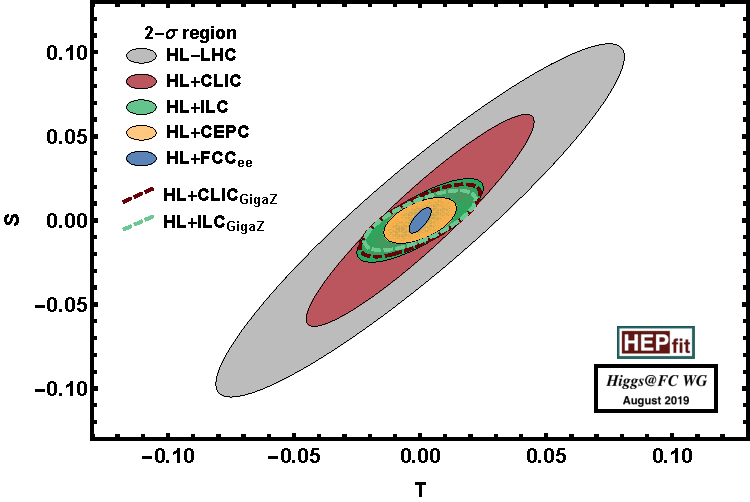
\includegraphics[width=.7\linewidth]{\main/ewksection/img/STplot_2sigma_noIntr}
    \caption{Expected uncertainty contour for the $S$ and $T$ parameters for various colliders in their first energy stage. For \ILC and \CLIC the projections are shown with and without a dedicated running at the $Z$-pole. 
    \label{fig:oblique}}
\end{figure}

In addition to measurements that probe the \ew sector of the SM, there are also several approaches at low-energy which provide interesting and complementary information. 
The forward-backward asymmetry $A_{FB}^{b}$ for the production of $b$ quarks measured at zero polarisation disagrees with the SM prediction 
by $2.3\,\sigma$~\cite{Tanabashi:2018oca}.
There is also a long-standing discrepancy of about $3\sigma$ between the value for the weak mixing angle, $\sintheta$ measured at LEP/SLC,
and that measured in neutrino deep-inelastic scattering by the NuTeV experiment~\cite{Zeller:2001hh}. The discrepancy may well be due to nuclear effects in the latter measurement~\cite{Beneke:2007zg}. The DUNE~\cite{Abi:2018dnh} experiment, primarily designed to measure the neutrino oscillations, plans to measure the $\sintheta$ with a precision of about 1\% using its near detector. This should clarify the discrepancy further and serve as a complementary probe for the $Z$-boson couplings to neutrinos at low energies $\sqrt{s} \ll M_Z$.  The electron-ion collider (EIC~\cite{Accardi:2012qut}), planned in the US, also plans to measure the dependence of $\sintheta$ on $Q^2$ in the range $Q^2\sim 10-70$~GeV$^2$ using polarised electrons scattered off unpolarised deuterons with a precision better than 1\%.

QED is the world's most precisely tested theory. The most impressive comparison between data and theory is the anomalous magnetic moment of the electron, $(g_e-2)$, ~\cite{Odom:2006zz,Gabrielse:2006gg} which has been measured with a precision of one part in $10^{12}$ and is found to agree with theoretical calculations performed up to order $\alpha^{5}$ (\cite{Volkov:2017xaq} and references therein). For the muon $(g_\mu-2)$, however, there is a $3-4\,\sigma$ discrepancy~\cite{Blum:2013xva,Jegerlehner:2018zrj} between theory and experiment which could hint at new physics breaking lepton universality. A new experiment is now running at FNAL to clarify the situation~\cite{Grange:2015fou}, aiming at a precision of $1.6\times 10^{-10}$ ($4\times$ better than the current precision). The uncertainty on the theoretical calculation is $\sim 5\times 10^{-10}$ and the largest source comes from hadronic contributions. The MuonE experiment~\cite{Abbiendi:2016xup} at CERN plans to make measurements of high-energy muons ($E=150$~GeV) scattering on atomic electrons ($\mu e\to \mu e$) to constrain the hadronic contributions to the theoretical value for $g_\mu$.

The fine structure constant at $M_Z$ is currently measured as $1/\alpha=128.952 \pm 0.014$, see Ref.~\cite{PhysRevD.98.030001}. 
Based on future measurements at BES III, Belle II and VHEP-2000, it should be possible to reduce it to $\pm 0.006$~\cite{Blondel:2019vdq}. 
It has been estimated that it can be reduced to $\pm 0.004$ by measuring the forward-backward asymmetries for 
$e^+e^- \to \mu^+\mu^-$ production versus $\sqrt{s}$ near $M_Z$ using 40~\iab of data~\cite{Janot:2015gjr} with \FCCee. The current uncertainty on $\alpha=\pm 0.014$ limits the precision of the \ew precision tests when the experimental precision on $M_W$ is reduced to below 8~MeV as expected possibly with \HLLHC but definitely at future $\epem$ colliders.

Tests of QED have so far been restricted mostly to the perturbative regime but already in the first half of the 20$^{\rm th}$ century it was pointed out that there is also a strong-field-limit in QED, where QED becomes non-perturbative~\cite{Sauter:1931zz,Heisenberg:1935qt}. This becomes relevant when the electrical field, seen by an electron, attains a value close to the Schwinger field~\cite{Schwinger:1951nm}. Several proposals exist to probe this regime with a high energy electron beam and a high-power laser using the AWAKE plasma wakefield accelerator at CERN~\cite{Caldwell:2018atq}, the European XFEL in Germany~\cite{Altarelli:2006zza}, or the FACET facility at SLAC~\cite{SLAC:2016van}. Previous experiments at SLAC and CERN did not quite reach the critical field value~\cite{Burke:1997ew,Andersen:2012ea}. The proposed new experiments will probe QED in the critical field regime, which is of relevance for instance for astrophysical phenomena (for instance magnetars~\cite{Kouveliotou:1998ze}), atoms with $Z>137$~\cite{pomeranchuk} and for high energy $e^+e^-$ colliders~\cite{Bell:1987rw, Blankenbecler:1988te}. 

\subsection{Higgs boson physics}
\label{sec:higgsfuture}

\subsubsection*{The Higgs boson couplings}
One of the most important open points after the discovery of the 125 GeV scalar at the LHC is how this particle couples to the known fermions and bosons, compared to the uniquely determined predictions from the Standard Model. Deviations in data from theory expectations would definitively indicate New Physics (NP), going Beyond the Standard Model (BSM), and as argued earlier in this chapter, they are a direct measure of the fine-tuning. 

Higgs boson couplings can be determined from the measurement of rates of events with given final states, which using the fact that the Higgs width is very small, can be expressed in terms of production cross sections times the decay branching fractions.

A simple yet powerful method to parameterise possible deviations from SM couplings is the so-called $\kappa$-framework ~\cite{LHCHiggsCrossSectionWorkingGroup:2012nn,LHCHXSWG3}.
In this framework, the deviations of SM Higgs boson couplings are parameterised through rescaling factors, the $\kappa_{i}$, which are defined as the ratios of the extracted couplings of the Higgs bosons to particles $i$ ($i=W, Z, \gamma, b, \tau,...$) to their corresponding values as predicted by the Standard Model.
Hence, the SM case is recovered by taking $\kappa_{i}$ = 1, for all particles $i$. This interpretation framework has the significant advantage of being extremely simple in its experimental implementation as well as of not needing any additional prediction from theory beyond those in the SM. This simplicity comes at a price; away from $\kappa=1$ the $\kappa$-framework violates gauge invariance. It is therefore a tool to indicate deviations from the standard model, but not to diagnose their cause.
The $\kappa$-framework can also be extended to probe new Higgs boson interactions, such as for instance, those of the Higgs boson with lighter BSM states. In this case, the total Higgs boson width, $\Gamma_H$ increases, and hence the branching fractions to SM final states are altered with respect to the SM predictions.  As discussed in Sec.~\ref{sec:ewkintro} Higgs boson decays to BSM particles can be separated in two classes: decays into invisible particles (with branching ratio \BRinv), and decays into all other untagged particles  (with branching ratio \BRunt).

The $\kappa$-framework, however,  by construction, does not parametrise possible effects coming from different Lorentz structures and/or the energy dependence in the Higgs couplings. Such effects could generically arise from the existence of NP at higher scales and could lead not only to changes in the predicted rates, but also in distributions. An efficient, robust and predictive parametrisation of these effects can be obtained  by extending the SM to an effective field theory, i.e. by including higher dimensional interactions which respect the SM symmetries and are suppressed by a scale $\Lambda$. A plausible class of such effective Lagrangians is the so-called SMEFT, which can be expressed as a polynomial of gauge invariant operators 
 organised as an expansion in inverse powers of $\Lambda, {\cal L}_{d}= \sum_{i}  c_{i}^{(d)} {\cal O}_{i}^{(d)}/\Lambda^{d-4}\, $.
The {\em Wilson  coefficients} $c_i^{(d)}$ encode the virtual effects of the heavy new physics in low-energy observables. Their precise form in terms of masses and couplings of the new particles can be obtained via {\it matching} with an ultraviolet (UV) completion of the SM, or inferred using {\it power-counting} rules. New physics effects start at dimension $d=6$ for which  a complete basis of operators is known. When considering the EW observables,  one can reasonably focus on a relatively small subset of operators, involving Higgs-boson, gauge-boson and fermion fields.
In the study presented here, {\it Neutral Diagonality} (ND) is assumed for flavour, which implies no flavour-changing couplings to the Higgs and Z boson.
In addition, in the fermion sector, only the 2nd and 3rd generation fermions are considered here, and their operators are treated independently. These assumptions give rise to modifications to the Higgs self-interaction, Higgs coupling to vector bosons, trilinear gauge couplings, Yukawa couplings to fermions, and vector couplings to fermions, for a total of 30 independent parameters.  

This scenario can be used to study the sensitivity at future colliders to general departures from the SM in the global fit to EWPO, Higgs boson rates and diboson production.  
%BH: I removed this below as I think we should show the more general EFT plot. 
%In fact, it is practical and useful to consider the case of idealised, {\it perfect EW} constraints, i.e. that any new physics contributions to the EWPO are bounded to be exactly zero. Considering further that SM theory uncertainties on EWPO are negligible, one can isolate the effect of the SM theory uncertainties in Higgs processes in the fit.  This series of assumptions leaves 12 parameters that can be expressed in terms of effective couplings.
%\BH{I am not quite sure about the above discussion on EWPO, I think it gives too much emphasis to it here and also as I suggest to use a different EFT figure I would shorten this. We can make a statement later (in words) what the EWPO do in the fit. }

Studies of the impact of future collider projects on the Higgs boson coupling precision have been made in both $\kappa$ and SMEFT frameworks by the \textit{Higgs@FutureCollider} working group~\cite{deBlas:2019rxi}, and are the basis of the results presented in the following.

Figure \ref{fig:Kappa3Summary} shows the expected precision of the $\kappa_i$ parameters for various future colliders~\cite{deBlas:2019rxi}, all combined with the expected \HLLHC results \cite{Cepeda:2019klc}. 
The Higgs width, $\Gamma_H$, is left free in the fit, and for hadron colliders a constraint $|\kappa_V|\leq 1$ is applied as the width is otherwise not constrained.
In all cases, experimental statistical and systematic uncertainties are included. For hadron colliders uncertainties on the Higgs production cross section are included. For decay branching ratios only the parametric uncertainties are included while the intrinsic uncertainties are neglected, see discussion in Ref.~\cite{deBlas:2019rxi} and Sec.~\ref{sec:ewktheory}.

\begin{figure}[t]
\centering
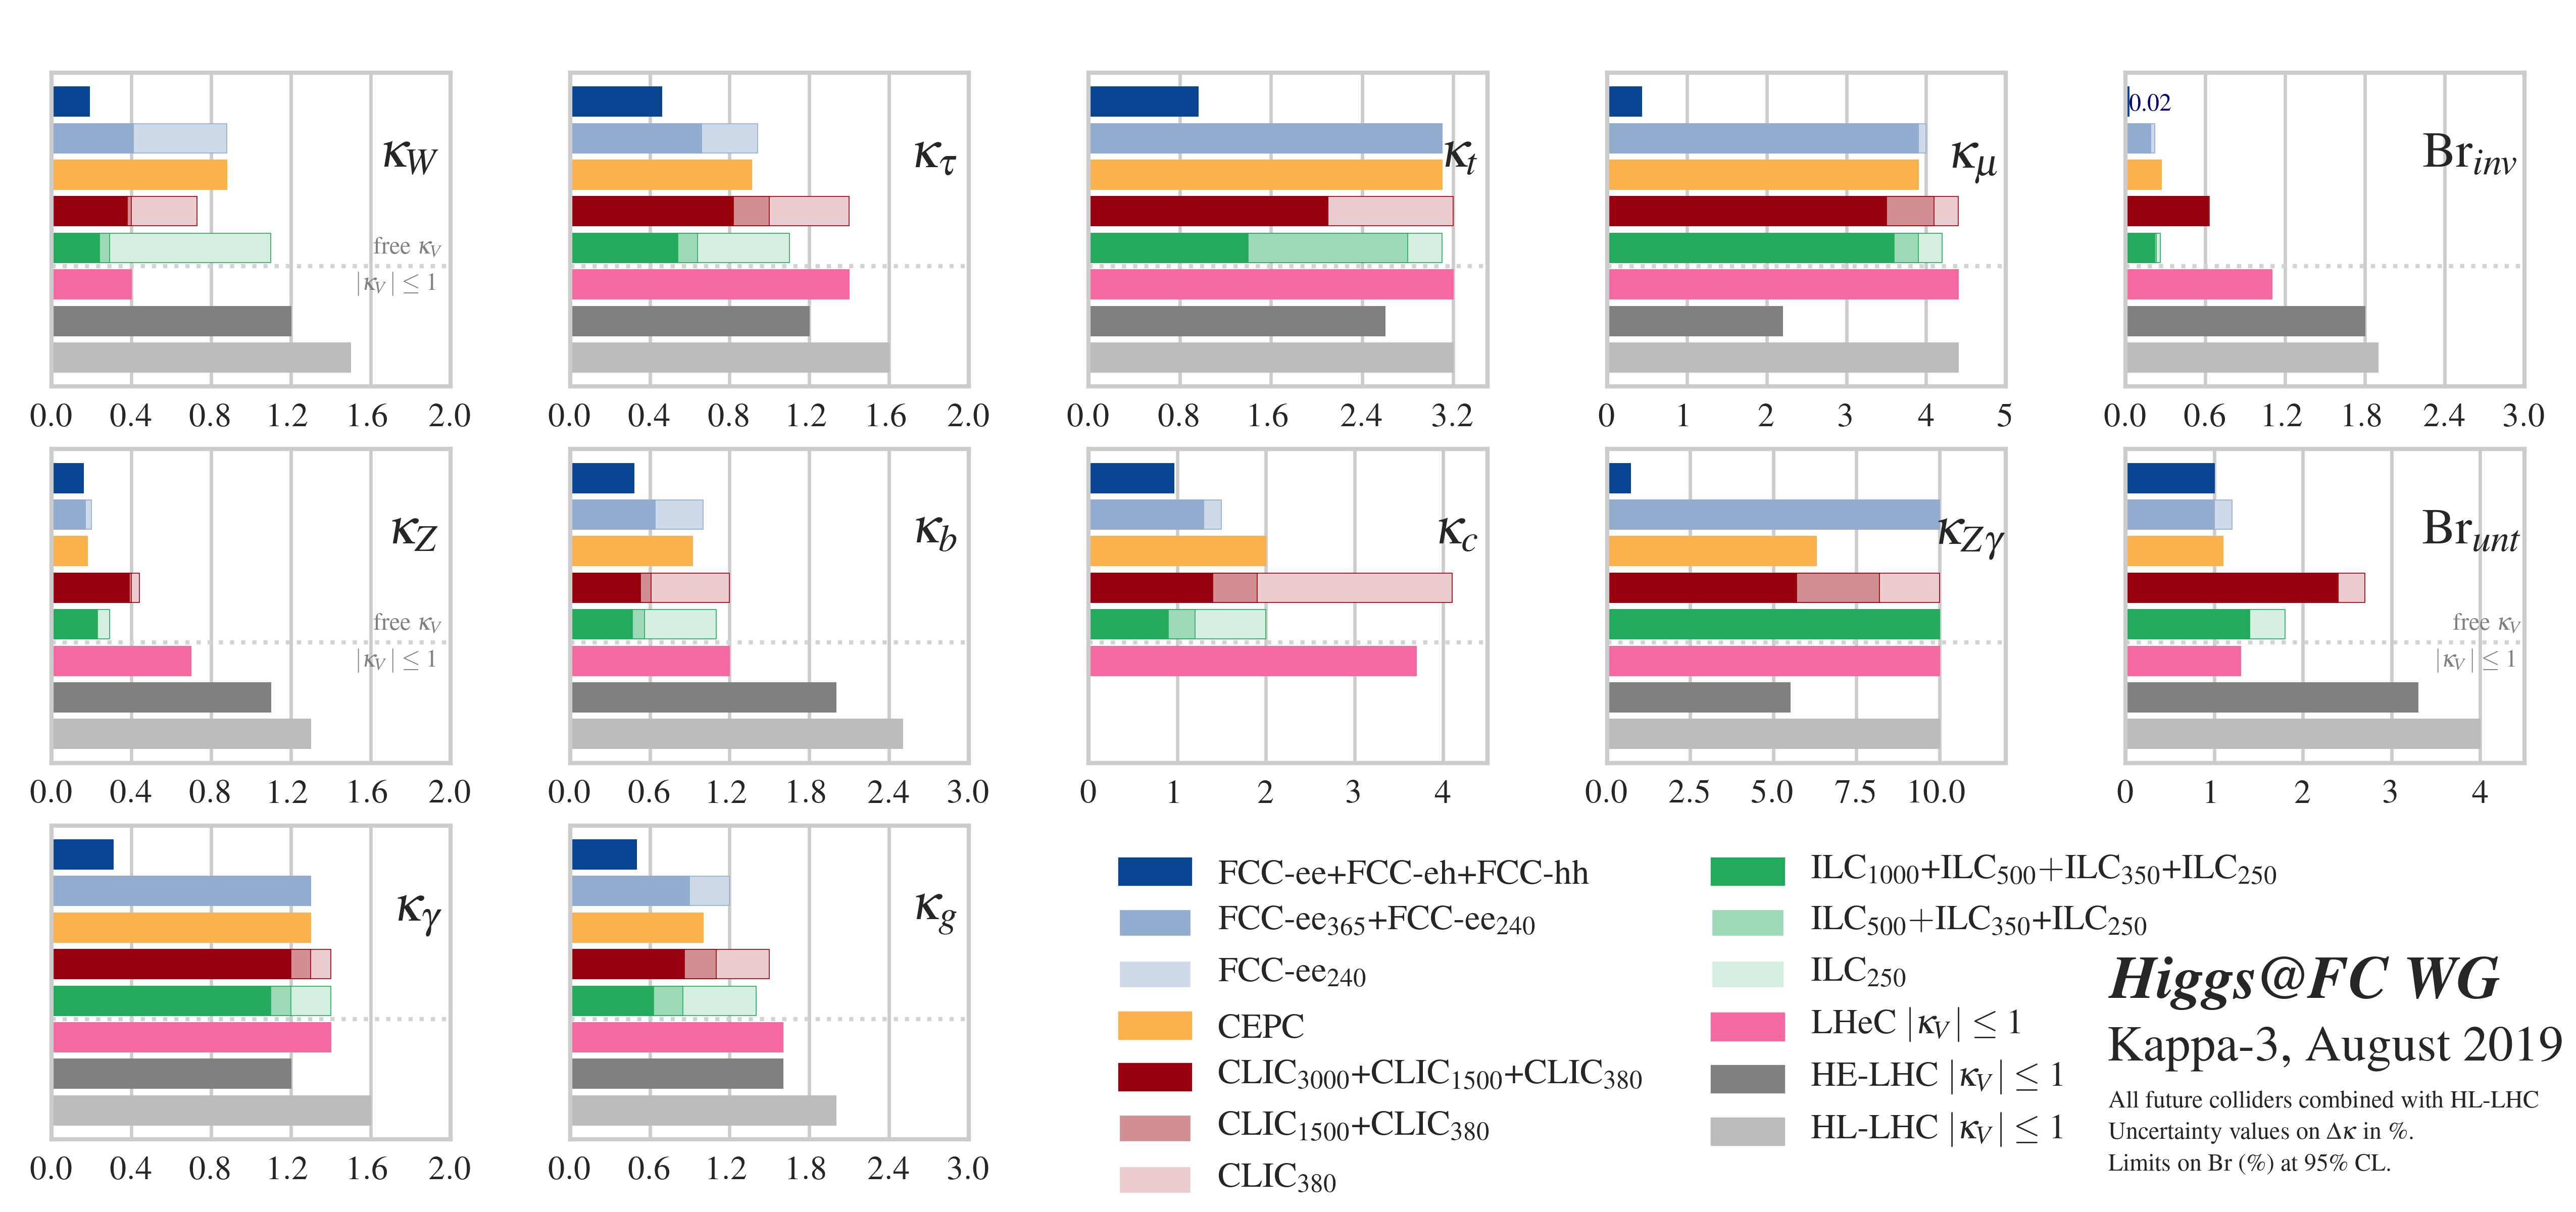
\includegraphics[width=0.9\linewidth]{\main/ewksection/img/Figure2Kappa3WithILC1000.png}
\caption{\label{fig:Kappa3Summary}
Expected relative precision of the $\kappa$ parameters and 95\% CL upper limits on the branching ratios to invisible and untagged particles for the various colliders. All values are given in \%. For the hadron colliders, a constraint $|\kappa_V|\leq 1$ is applied, and all future colliders are combined with \HLLHC. Figure is from Ref.~\cite{deBlas:2019rxi}.
}
\end{figure}

At the \HLLHC the Higgs boson couplings can be determined with an accuracy of ${\cal O}(1-3\%)$ in most cases, under the assumption $|\kappa_V| \leq 1$. Ratios of couplings are (mostly) model independent, and an accuracy of ${\cal O}(1-3\%)$ is expected in many cases~\cite{Cepeda:2019klc}.
Based on analyses of final states with large $\etmiss$, produced in Higgs VBF and VH (V=W and Z) processes, BR$_\textrm{inv}$ values of 1.9\% will be probed at 95\% CL. The constraint from the $\kappa$-fit on the BR to untagged final states is 4.0\% at 95\% CL. The \HELHC improves the precision typically by a factor of two, although much of the improvement comes from the assumption 
of a further reduction by a factor of two in the theoretical uncertainty, scheme $S2^{\prime}$~\cite{Cepeda:2019klc}.

Lepton colliders allow a measurement of the ZH total production cross section, independently of its decay making use of the collision energy constraint. This measurement, together with measurements where the decay products of the Higgs boson are identified, can be interpreted as a nearly model-independent measurement of the total decay width. Therefore the constraint $|\kappa_V| \leq 1$, used for hadron colliders, is not needed for lepton colliders. 

Future $e^+e^-$ colliders improve the accuracy on Higgs coupling determination typically by factors between 2 and 10, except for $\kappa_t$, $\kappa_\gamma$, $\kappa_\mu$ and $\kappa_{Z\gamma}$ where no substantial improvement compared to \HLLHC is seen. \LHeC achieves a significant improvement for $\kappa_W$, $\kappa_Z$ and $\kappa_b$.
At $e^+e^-$  colliders, the couplings to vector bosons will be probed with a few 0.1\% accuracy. Higgs boson couplings to b-quarks can be measured with an accuracy between 0.5\% and 1.0\%, a factor of $2-4$ better than at the \HLLHC.  The coupling to the charm quark, not easily accessible at \HLLHC, is expected to be measured with an accuracy of ${\cal O}(1\%)$. The various $e^+e^-$ colliders do not differ significantly in their initial energy stages. 

The rate of rare Higgs boson decays such as $H\to \mu^+\mu^-$ that allows the study of the second generation lepton couplings, will be best measured by \HLLHC with an accuracy of about 4\%. 

When \FCCee is combined with \FCCeh and \FCChh a further significant improvement is seen, particularly for couplings to top quark, muons, photons and $Z\gamma$ where \FCChh will benefit from very large event samples. The improvement in $\kappa_W$ comes primarily from \FCCeh. A study of various other combination of aspects of the \FCC programme is documented in Ref.~\cite{deBlas:2019rxi}. 
 
The sensitivity of the Higgs branching ratio to BSM invisible final states is predicted to be improved by a factor 3 (CLIC) to 10 (\FCCee, \ILC) with respect to \HLLHC. For \FCChh a sensitivity to branching ratios as small as $0.025\%$ is expected to be achieved. Branching ratios to untagged decays are typically probed with a precision of $(1-2)\%$.

In Fig.~\ref{fig:EFT-results}, the results of the fit corresponding on the EFT benchmark, expressed in terms of effective couplings, are shown. Also shown are the constraints on the trilinear gauge boson coupling parameters ($\delta g_{1Z}$, $\delta \kappa_\gamma$ and $\lambda$). Again, it is seen that the $e^+e^-$ colliders improve most parameters by about factors of 5-10. The exceptions are the the coupling parameters related to top, $Z\gamma$ and $\mu$ couplings. The sensitivity of the different types of $\epem$ colliders is similar in their first stages. The improvements seen for \HELHC and LHeC are more modest.
For the $Z$ and $W$ a sensitivity below 0.3\% can be achieved by \ILC, \CLIC and \FCC. At this precision, the uncertainty is potentially limited by the intrinsic theory uncertainties which is not considered here (see discussion in Sec.~\ref{sec:ewktheory}). For fermions, the best sensitivity is reached for $b$-quarks and $\tau$-leptons, and it is about 0.5\%. %In general, the conclusions are rather similar to those reached with the $\kappa$-framework, except that the relative 

%\begin{figure}[t]
%\centering
%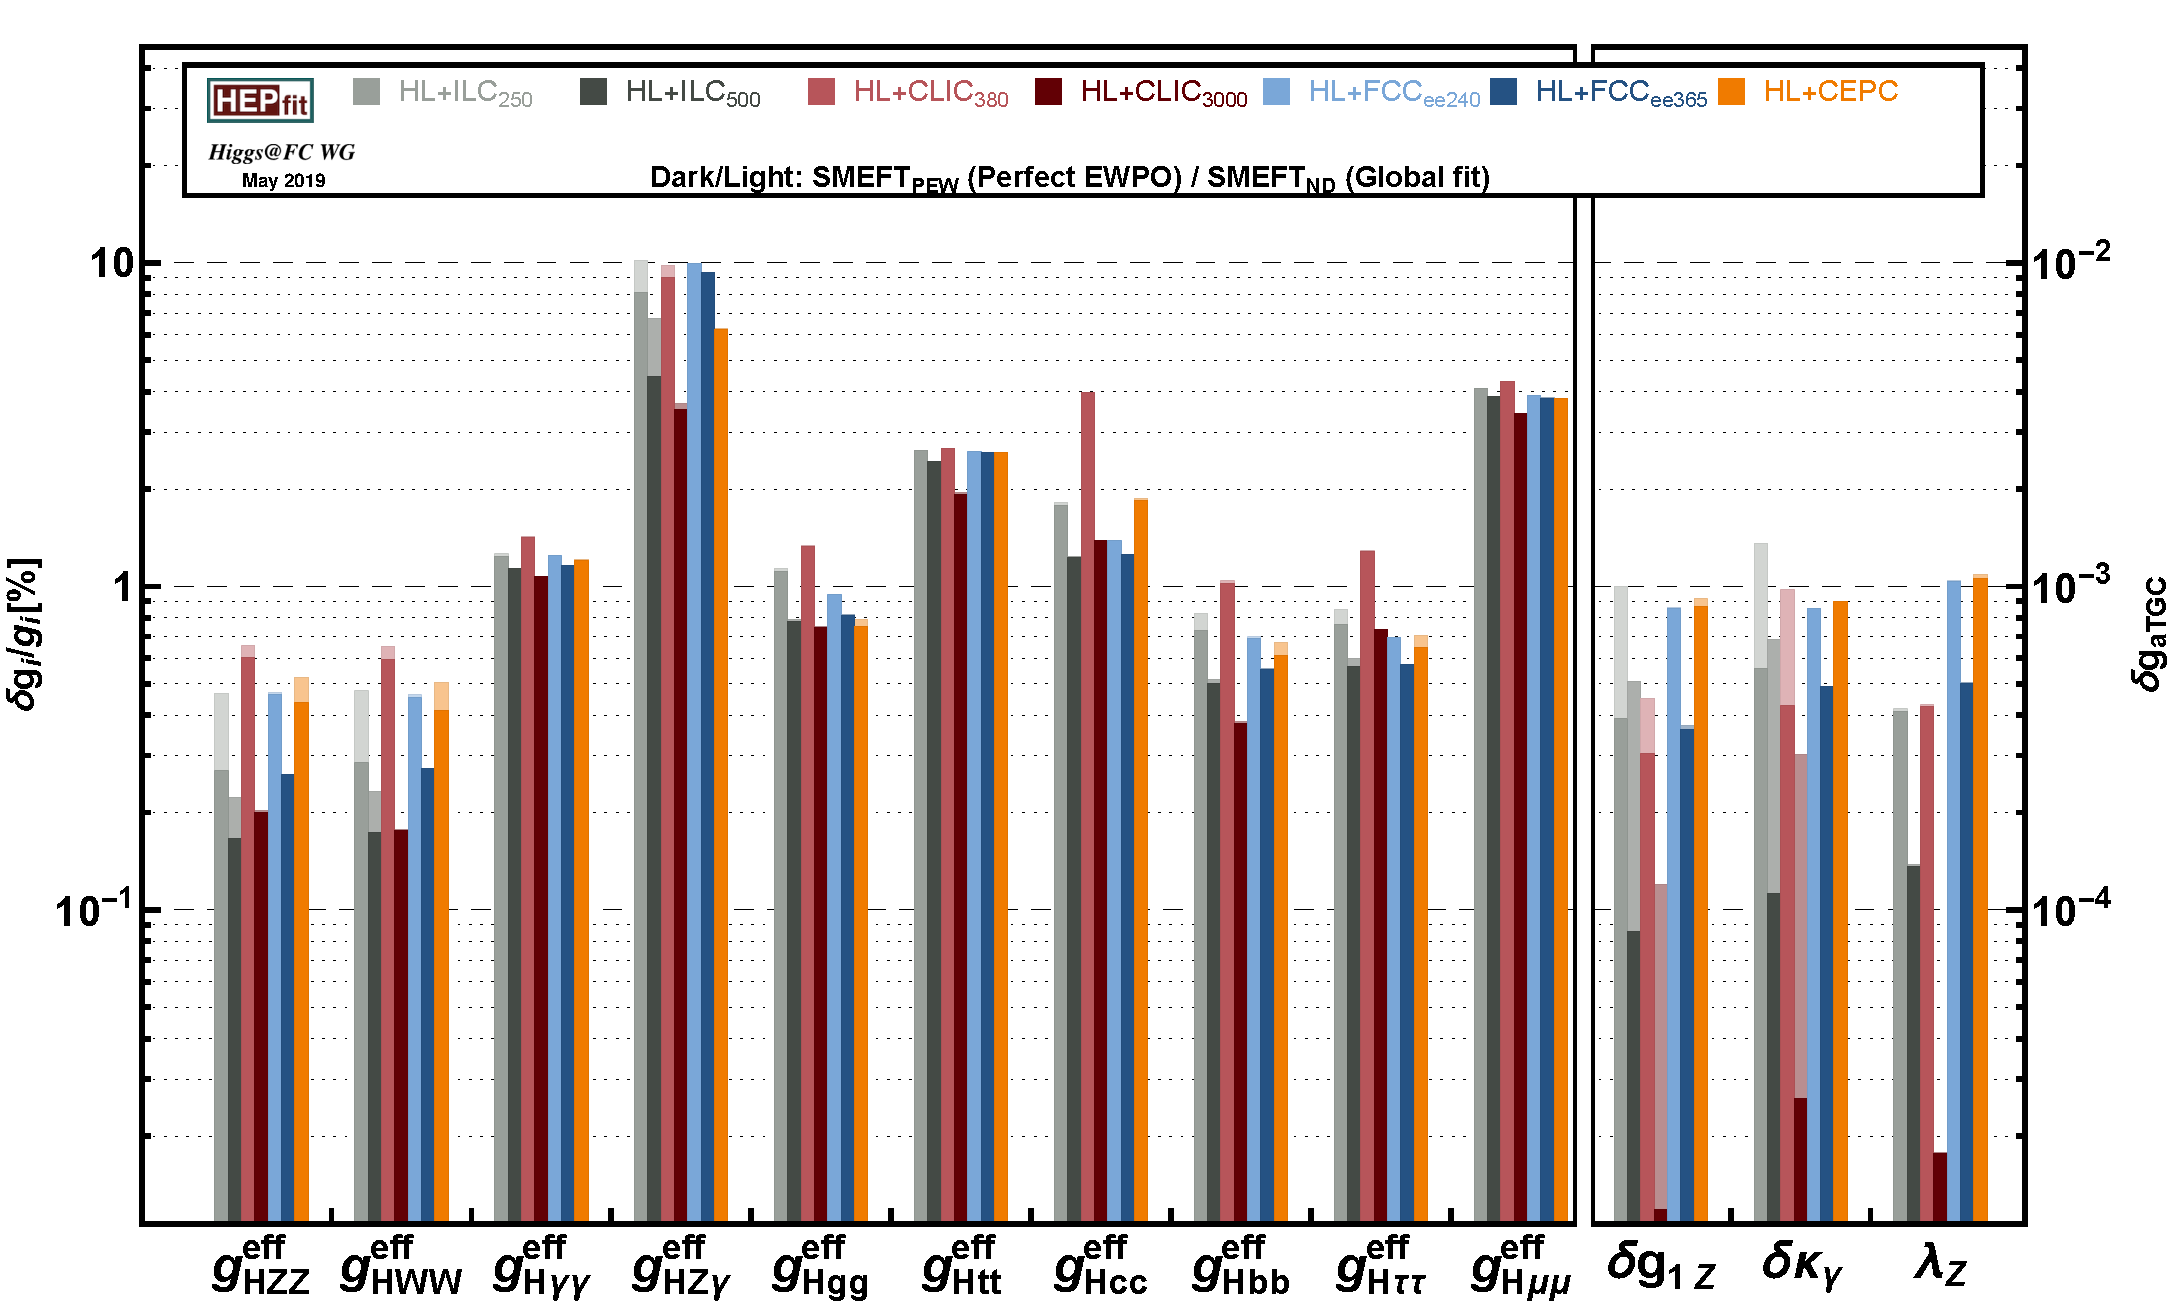
\includegraphics[width=0.9\linewidth]{\main/ewksection/img/Global_vs_Perfect_flat.pdf}
%\caption{\label{fig:EFT-results}
%68$\%$ probability reach on Higgs couplings and aTGC at the different lepton colliders from the Global fit SMEFT$_{\rm ND}$, compared with the results obtained assuming infinite precision for the EWPO (scenario SMEFT$_{PEW}$). For details, see \cite{deBlas:2019rxi}.
%\BH{WHy show this figure which highlights the EWK precision data? I think we should show the main result instead and put this figure in now, and added a discussion of it}}
%\end{figure}

\begin{figure}[t]
\centering
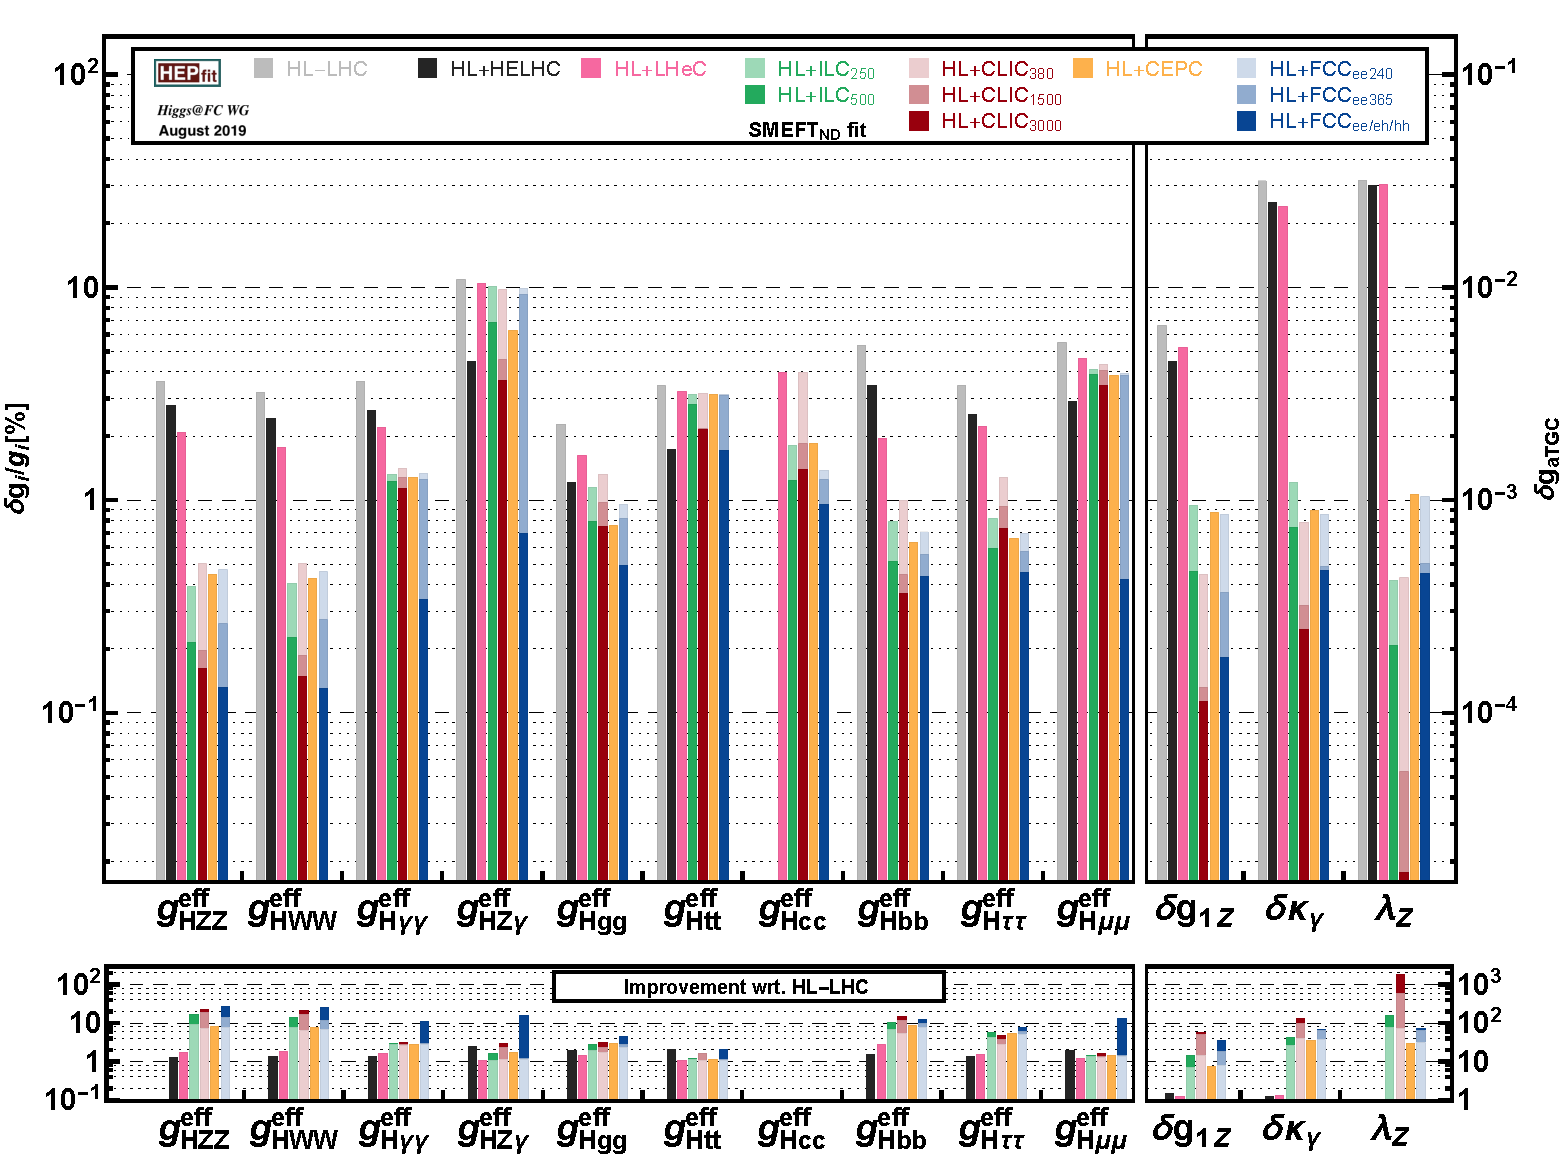
\includegraphics[width=0.9\linewidth]{\main/ewksection/img/Global_noH3_Aug}
\caption{\label{fig:EFT-results}
68$\%$ probability reach on Higgs couplings and aTGC at the different future colliders from the Global fit SMEFT$_{\rm ND}$. In the lower panel the improvement factor with respect to the \HLLHC is shown for each parameter. For details, see Ref.~\cite{deBlas:2019rxi}.
}
\end{figure}

\subsubsection*{The Higgs boson self-coupling}
The Higgs field is responsible for the spontaneous breaking of the \ew symmetry, and for the generation of all the SM particle masses.
Within the SM, the associated Higgs potential is characterised by one parameter, $\lambda$, that can be inferred from the experimental measurements of the Fermi constant $G_F$ and of the Higgs mass $m_H$,  (see Eq.~\ref{eq:SMpotential}). Beyond the SM, the parameter $\lambda$ is unconstrained experimentally, and could show particularly sizeable departures from the SM prediction. The determination of parameters related to the Higgs potential is therefore a high priority goal of the physics programme of all future colliders. 

The most direct way to assess the Higgs boson self-interaction and  in particular $\lambda_3$, is through the measurement of processes that feature two Higgs bosons in the final state.  At hadron colliders,  double Higgs boson production cross section is dominated by gluon fusion, $gg\to HH$, while at lepton colliders it proceeds via double Higgs-strahlung,  $e^+e^-\to ZHH$, particularly relevant at low energies, or via vector boson fusion (VBF), $e^+e^-\to HH\nu_e\bar{\nu}_e$, more important at centre-of-mass energies of 1\,TeV and above. 

For the \HLLHC, the cross section is predicted to be about three orders of magnitude smaller than the single Higgs production, which makes the double Higgs boson final state a challenging process to observe. The analysis relies on the combination of the $b\bar{b}\gamma\gamma$ and $b\bar{b}\tau\tau$ decay channels to reach about four standard deviation evidence for double Higgs production at \HLLHC (see Table~55 and Fig.~65 of Ref~\cite{Cepeda:2019klc}). This corresponds to an accuracy on $\kappa_3 = \lambda_3$/$\lambda_3^{\rm SM}$ of about 50\%.

Higgs self-interactions also affect, at higher orders, the single Higgs processes~\cite{McCullough:2013rea,Degrassi:2016wml,Bizon:2016wgr}  and even the \ew precision observables~\cite{vanderBij:1985ww, Degrassi:2017ucl, Kribs:2017znd}. Therefore, single-Higgs boson production measurements can also be used to extract the Higgs self-coupling strength.

Figure \ref{fig:h3-summary} shows the uncertainty expected on the measurement of $\kappa_3$ at the various proposed future colliders, in combination with the expectation from \HLLHC. The results have been obtained by studying the determination of $\kappa_3$ that can be obtained from single and double Higgs boson production processes using the EFT framework (see above). It is found that, when accessible, the HH channel plays a pivotal role in constraining the trilinear self-coupling, as its addition to the fit allows to fully exploit single Higgs boson measurements to put severe constraints on the possible deviations of the other Higgs couplings, e.g.,  the top-quark Yukawa.  Details of this study are presented and discussed in Ref. \cite{deBlas:2019rxi}.

\begin{figure}[!ht]
\centering
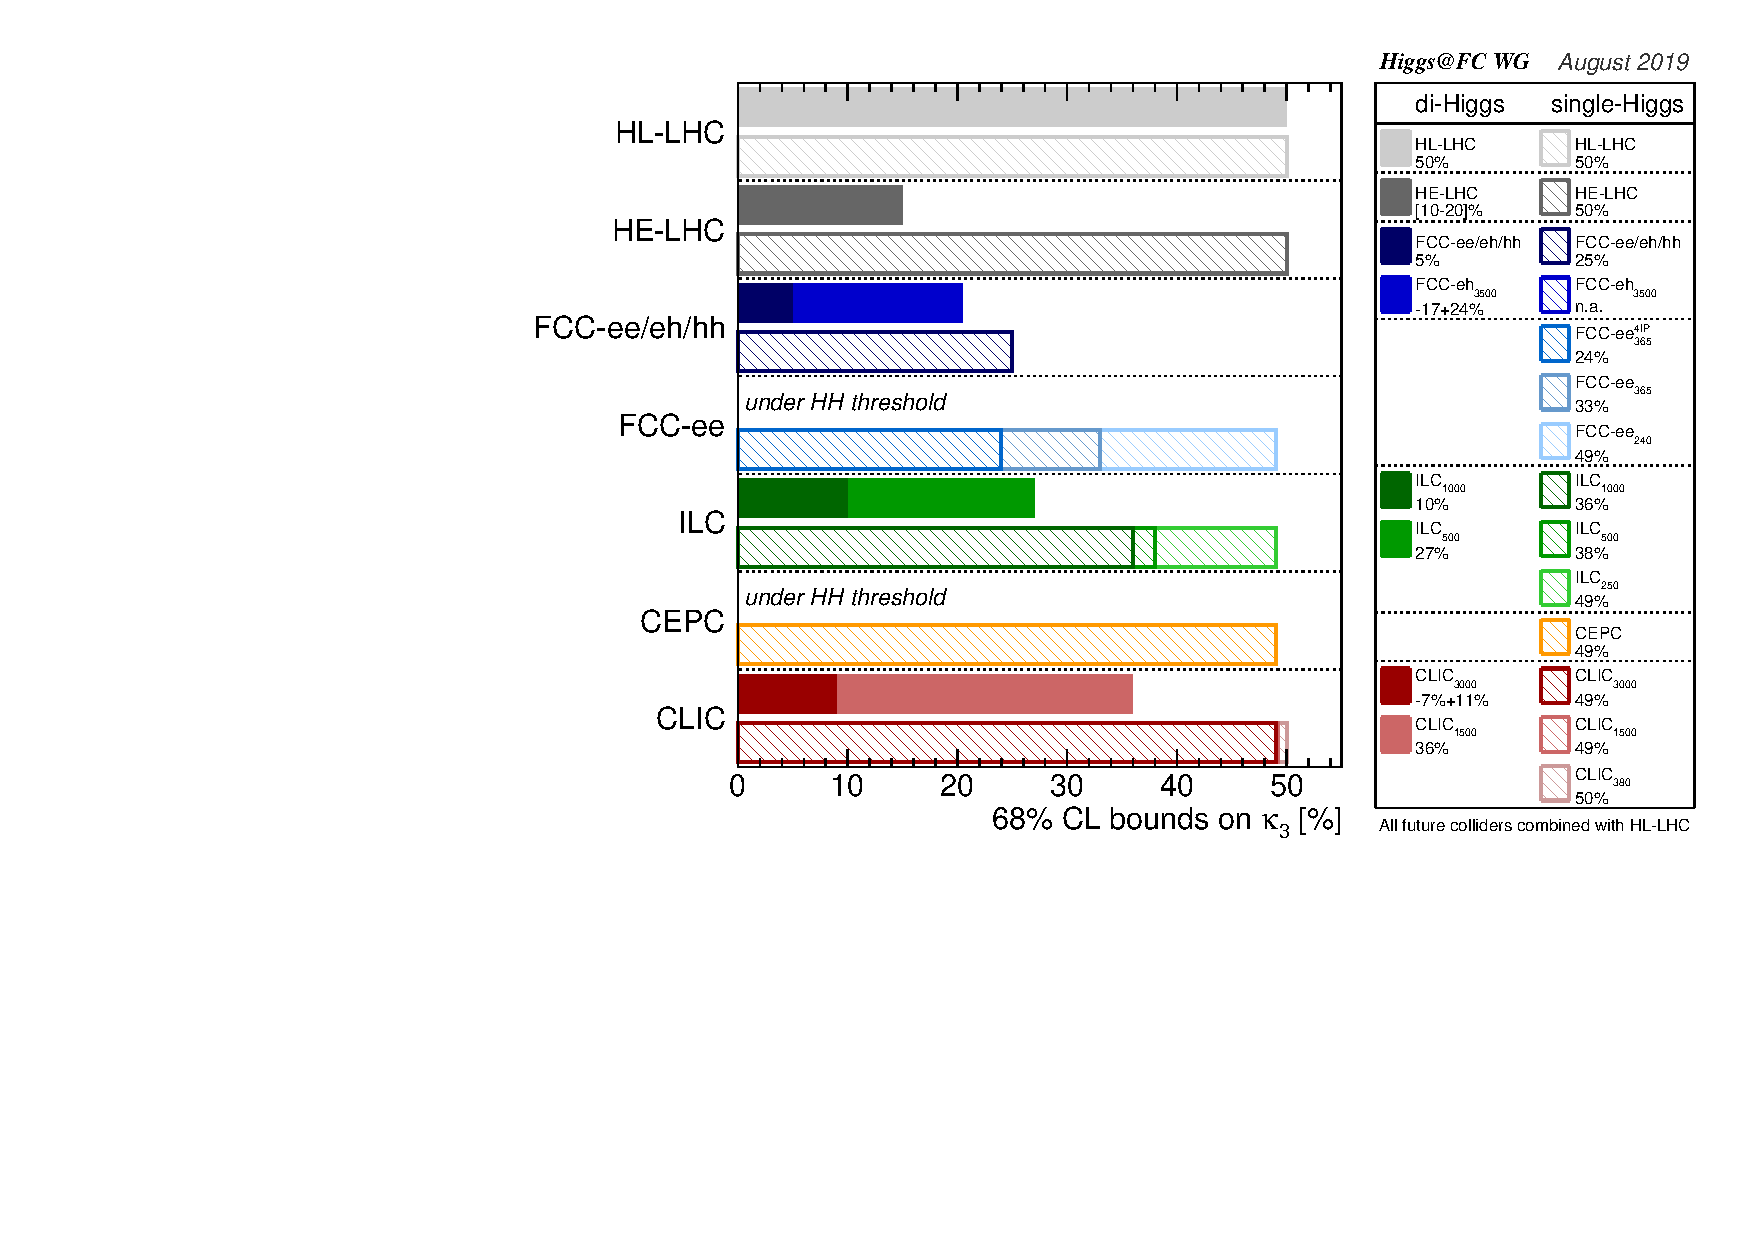
\includegraphics[width=.8\linewidth]{\main/ewksection/img/PrecisionKappaLambda_Summary_4methods_2}
\caption{\label{fig:h3-summary}
Sensitivity at 68\% probability on the Higgs self-coupling parameter $\kappa_3$ at the various Future Colliders. All the numbers reported correspond to a simplified combination of the considered collider with \HLLHC which is approximated by a 50\% constraint on $\kappa_3$.
For each future collider, the result from the single-H from a global fit, and double-H are shown separately.
For \FCCee and \CEPC, double-H production is not available due to the too low $\sqrt{s}$ value.
}
\end{figure}

CLIC at $\sqrt s \geq 1$~TeV can extract $\kappa_3$ with a precision of about than 10\%. This accuracy would reduce to about 30\% for lower center of mass energies and for \ILC, but it is still interesting as different processes are probed which can be affected differently by new physics contributions. 
Circular $e^+e^-$ colliders have insufficient energy to produce two Higgs bosons, and rely on the global fit of single-$H$ analyses, dominated by the high precision estimated for the $ZH$ cross section measurement. In this case, an accuracy of about 34\% can be achieved by \FCCee.
\HELHC and \FCChh, can extract $\kappa_3$ with an accuracy of 15\% and 5\% using $HH$ production, respectively. It was estimated that \ILC at $\sqrt{s}=1$~TeV will also achieve a precision of 10\%~\cite{ilc1000}.

At \FCChh, a $2\sigma$ sensitivity to the quartic coupling, $\lambda_4$, is also expected. 

\subsection{Theoretical developments}
\label{sec:ewktheory}
The expected increase of precision in the measurements of EW observables at future colliders will demand a substantial improvement in the accuracy of theoretical predictions, (see also \cite{Blondel:2019qlh}). In this subsection, the needs are motivated and estimates are provided on what could be achieved based on the developments in the field in the last years, for both $e^+ e^-$ and $pp$ colliders. Figure~\ref{fig:higgsnow} has already shown that the dominant uncertainties in most Higgs couplings at the \HLLHC 
are theoretical, even after assuming a factor of two improvement 
with respect to the current state of the art. Higgs couplings will be approaching the percent level at \HLLHC.
At the $e^+e^-$ Higgs factories detailed measurements of the \ew Higgs production cross sections and (independently) of the decay branching ratios will be performed. Higgs couplings will be probed at at approaching the per mille level.
At $e^+e^-$ colliders, a campaign of \ew  measurements at the $Z$-pole and at the $WW$ threshold is foreseen.  
The increase  in the number of $Z$ and $WW$ events with respect to LEP/SLD, as shown in Fig.~\ref{fig:ewkprogramme}, indicates that statistical errors will decrease by as much as two orders of magnitude at the future machines. As a consequence of this increased statistical precision, the requirements on the theoretical errors for EWPO~\cite{Blondel:2018mad} are even more stringent than for precision Higgs physics.

To interpret these precise results significant theoretical improvements  in several directions are required.  The first  is the increase of the accuracy of fixed order computations of inclusive quantities, e.g.  from next-to-leading-order (NLO) to next-to-next-to-leading order (NNLO) and beyond. This reduces the so-called intrinsic uncertainties, i.e. those corresponding to the left-over unknown higher order terms in the perturbative expansion. Another important element is the accuracy in the logarithmic resummations that are needed to account for effects of multiple gluon or photon radiation in a large class of observables. In this case, different techniques and results are available, some numerical and some analytic, of different accuracy (from next-to-leading log (NLL) to next-to-next-to-leading log (NNLL) and beyond) and applicability. Improvements in the resummed predictions as well as their matching to fixed-order calculations of the highest accuracy will be needed also in the form of fully exclusive Monte Carlo generators that can be directly employed by the experimental collaborations. Finally, a reduction of the so-called parametric uncertainties, i.e. those coming from the imperfect knowledge of the input parameters, will also call for improvements in the theoretical predictions related to their extraction from data. For example, for Higgs decay processes, the  principal parametric uncertainties are the Higgs mass and the quark masses ($m_t,m_b,\ldots$) and the value of $\alpha_s(M_Z)$~\cite{Lepage:2014fla}. 
For general \ew processes there are parametric uncertainties associated with $\alpha(M_Z),M_Z,M_W$.  For hadronic production, uncertainties from parton distribution functions also contribute.
\begin{table}
\begin{center}
\caption{Current and projected errors on input parameters. Where a lower bound 
is given on the projected uncertainties, the value is future machine dependent, see 
Fig.~\ref{fig:ewkpar}.}
\label{PUncertainties}
\begin{tabular}{|l|l|l|l|}
\hline
Error on&  Current value & Projected value & Uncertainty on  quantity\\
parameter &  ref.\cite{deFlorian:2016spz} & ref.\cite{Freitas:2019bre} & with projected value \\
\hline
$\delta M_H$  & 240~MeV & $>10$~MeV & $\Gamma_H(WW^*,ZZ^*),(0.1\%)$\\
$\delta m_t(m_t)$  & 1000~MeV & 50~MeV& \\
$\delta m_b(m_b)$  & 30~MeV & 13~MeV & $\Gamma_H(b \bar{b}),(0.6\%)$ \\
$\delta m_c$(3 GeV)  & 26~MeV & 10~MeV & $\Gamma_H(c \bar{c}),(1\%)$\\
$\delta M_Z$  & 2.1~MeV & $>0.1$~MeV & \\
$\delta M_W$  & 12~MeV & $>0.7$~MeV & \\
$\delta \alpha_S(M_Z)$  & $1.5\times 10^{-3}$ & $2\times 10^{-4}$& $\Gamma_H(gg),(0.5\%)$\\
$\delta \alpha(M_Z)$  & $10^{-4}$ &  $>5\times 10^{-5}$& \\
\hline
\end{tabular}
\end{center}
\end{table}

Observables in the SM are calculable in terms of a double expansion in 
$\alpha_W =g_W^2/(4 \pi) \sim 0.034$ and in $\alpha_S$, which at high scales becomes small, for example,  $\alpha_S(M_Z)\sim 0.118$. Given the relative size of the interactions,  QCD corrections where applicable,  are more important than the \ew ones. Yet, QCD corrections at NNLO $O(\alpha_S^2)$ are expected to be of similar size as NLO $O(\alpha_W)$ \ew corrections. In addition, because of the special nature of QCD renormalization group improved perturbation theory, 
the naive expectation that $O(\alpha_s)$ NLO predictions should have an intrinsic uncertainty of $O(\alpha_s^2) \simeq 1\%$ does not hold. In fact, to achieve $1\%$ precision in a QCD computation, a combination of a higher fixed--order and resummed results has to be computed. 

The interpretation of the \ew production measurements of $e^+ e^- \to ZH, e^+ e^-\to \nu \bar{\nu} H$ requires predictions including EW corrections starting at one loop and QCD corrections starting at two loops. Decay branching ratios require both QCD and \ew corrections starting at one loop. 

At hadron colliders, QCD corrections to the production mechanisms are the dominant effect and their imperfect knowledge provides the main source of uncertainty. This is already the case 
at HL-LHC where for all decay modes which are not statistically limited the dominant uncertainty 
is theoretical as shown in Fig.~\ref{fig:higgsnow}. In addition, in order to be directly usable in experimental analyses, results need to be accurate, fully differential and include matching with parton showers, in order to be available in the form a Monte Carlo generator.

In order to judge the plausibility of success in reaching the desired theoretical improvements it may be useful to look backwards and note what has been achieved in the last twenty years in the context of $pp$ colliders. 
At the end of the last millennium, systematic algorithms existed for calculating differential NLO results, and a handful of NNLO results for QCD corrections, i.e. inclusive single boson ($\gamma^*,W,Z,H$) production, and relatively small set of results at NLO EW. The general purpose Monte Carlo programs, Herwig\cite{Corcella:1999qn} and Pythia\cite{Sjostrand:2000wi}
evaluated all cross sections at leading order. And fits to parton distribution functions were provided without any attempt to quantify uncertainties. 

Since then a number of achievements have been made; the complete automation of calculations for multi-leg processes, the matching to parton showers up to NLO in both QCD and in EW (see e.g. Ref.~\cite{Frederix:2018nkq,Alwall:2014hca}), 
intensive development of systematic NNLO subtraction and slicing algorithms
%\cite{} 
allowing fully differential predictions to be made at NNLO
%~\cite{} 
for a number of ($2 \to 2$) processes, 
N$^{3}$LO calculations for $2 \to 1$ processes\cite{Mistlberger:2018etf}, now also including some differential information.
%~\cite{}
The calculation of DGLAP evolution kernels at N$^{2}$LO\cite{Vogt:2004mw,Moch:2004pa} has been furthere completed with partial results at higher loop order, and reached a large consensus on parton distributions with accompanying errors\cite{Butterworth:2015oua}. 

These technical advances have allowed predictions for the different mechanisms of Higgs boson production at $pp$ colliders. The results for the various mechanisms, gluon-gluon fusion (through a heavy quark loop), vector boson fusion, associated production with an \ew vector boson, associated production with a heavy quark pair, (top or bottom), and associated production with a top quark have already been shown in Fig.~\ref{fig:Higgs_XS_7-100TeV_HH}. The accuracy achieved has been reached as a result of the calculations, detailed in Table \ref{tab:StateofArt}.
\begin{table}
\begin{center}
\caption{State-of-the-art QCD corrections at fixed order for Higgs boson production in $pp$ collisions.  NLO EW corrections are known for all processes.  }
\label{tab:StateofArt}
\begin{tabular}{|l|l|l|l|}
\hline
Gluon fusion (effective theory)  & N$^{3}$LO & Total cross section & \cite{Mistlberger:2018etf,Dulat:2018rbf} \\
                                 & N$^{3}$LO & Rapidity distribution  & \cite{Dulat:2018bfe,Cieri:2018oms} \\
\hline 
Higgs + 1 jet (effective theory)   & NNLO & differential & \cite{Chen:2016zka}  \\
Higgs + 1 jet (full  theory)       & NLO  & differential & \cite{Jones:2018hbb} \\
\hline
Vector boson fusion   & NNLO (N$^{3}$LO) & differential (total) & \cite{Cruz-Martinez:2018dvl,Cacciari:2015jma,Figy:2007kv} (\cite{Dreyer:2016oyx})\\
\hline
$VH$   & NNLO & differential & \cite{Ferrera:2017zex,Caola:2017xuq} \\
\hline
$ttH$ production & NLO & differential  & \cite{Reina:2001sf,Beenakker:2002nc,Yu:2014cka} \\
$tHj$  production & NLO & differential  & \cite{Farina:2012xp,Demartin:2015uha} \\
\hline
\end{tabular}
\end{center}
\end{table}
%
Predictions for Higgs decay widths to various possible final state are also known at rather high precision, with uncertainties ranging from a few per mille ($bb,\tau\tau,\mu\mu,WW,ZZ$) to a few percent level ($\gamma\gamma,gg,\gamma Z$). 

A comprehensive list of the specific calculations which will be needed together with the development of new techniques in the context of EW physics at the future colliders cannot be presented here. However, the main challenges can be illustrated by discussing a few key examples. 

At $e^+e^-$ colliders running at the $Z$ pole, one expects that the fully inclusive $Z$ decay rates EW and EW-QCD three loop computations as well as the EW 2-loop calculation for off-shell $e^+e^- \to f\bar{f}$ will be needed.  These calculations are expected to be challenging but in line with expected progress in the field. In addition, conceptual work towards a sound extension of the definitions of pseudo-observables at the targeted accuracy will be necessary. 

For the $WW$ cross section scan at $e^+e^-$ colliders, the full NNLO EFT calculation for $e^+e^- \to WW$ is foreseen together with the determination of the leading 3-loop Coloumb-enhanced EFT corrections, achieving the targeted accuracy of $(1-4) \times 10^{-4}$ for $\sigma(WW)$ at threshold. 

Finally, for Higgs production at $e^+e^-$ colliders, the full EW 2-loop calculation for on-shell $e^+e^- \to ZH$ and the leading contributions to $e^+ e^-\to \nu \bar{\nu} H$ will be needed. Obtaining these results is in line with the expected developments in the field of multi-scale two-loop computations. In addition, Higgs decay widths into massless partons in 4-/5-loop QCD calculations are expected. 

At $pp$ colliders a concerted effort in multiple directions will be needed for better determination of the signal as well as backgrounds. The inclusion of higher-order corrections in QCD and mixed QCD/EW, the improvement on the accuracy of the parton shower algorithms in line with the accuracy achievable with analytic resummations, the definition of new more perturbatively stable observables, are being pursued. The relative importance of each of such improvements for a given observable will depend on the specific process under consideration. 

For $pp$ colliders, the uncertainties on the parton distribution functions also play an important role when comparing measured cross sections to theoretical predictions. For the HL-LHC they are expected to be reduced by a factor of two compared to the current precision, and an additional reduction by a factor of two is assumed for HE-LHC. These reductions are assumed to be possible with precise measurements of various $pp$ cross sections~\cite{Khalek:2018mdn}. For \FCChh the projections are mostly based on ratios of cross sections where the uncertainties should largely cancel. If an $ep$ collider is available such as \LHeC or \FCCeh, the uncertainties on e.g. Higgs coupling measurements at these hadron colliders can be further improved.

\section{Summary and conclusions}
There is a very rich programme of precision measurements to be made of the properties of the Higgs boson, and of the other particles and parameters that are relevant to the \ew force. Both \ew precision observables and Higgs couplings can be related directly to the naturalness problem, the problem of why the Higgs mass is unstable in the SM and whether there is new physics that stabilizes it at the \ew scale. 

Precise measurements of the $Z$ boson could be made at future $\epem$ colliders, in particular at circular colliders where $10^{12}$ $Z$-bosons would be available. At linear colliders a significant advance compared to the current precision is also expected, thanks in part to the polarisation that is available. The oblique parameters will be measured with a precision of $\sim 1\%$, about a factor 10 better than the current precision. Furthermore, several low-energy experiments are expected to also contribute to the precise determination of important parameters of the \ew aspects of the SM.

The precision measurements of Higgs boson couplings are sensitive to BSM physics as it can alter them from their SM values. The \HLLHC will vastly improve the precision on the Higgs boson coupling parameters from typically 15\% today to a few percent with the full dataset, assuming that the present theory uncertainties will be reduced by a factor of two.  A further large improvement can be achieved with future $e^+e^-$ colliders, which also have the novel and powerful ability to measure Higgs production without any assumptions on its decay. The sensitivities in their initial stages are rather comparable. The most precise coupling measurements (to $Z$ and $W$ bosons), are measured to 0.2-0.3\% depending in part on the precision that can be achieved for the theoretical calculations. Additionally, Higgs decays to invisible particles (e.g. dark matter candidates) can be constrained to values much better than 1\%. The measurement of the total width to within a few percent, possible at $e^+e^-$ colliders, will provide an important constraint on many new physics scenarios.

The Higgs self-coupling is currently unconstrained by data, and a deviation of $\sim 1$ from the SM value has potentially dramatic consequences for cosmology, in particular the Nature of the \ew phase transition that occurred in the early Universe. It can be measured to $\sim 50\%$ precision at \HLLHC, and ultimately a precision of 5-10\% could be reached at \FCChh at 100 TeV, \CLIC at 3 TeV or \ILC at 1 TeV. 

In summary, the \ew precision programme provides a complementary way to search for new fundamental particles, and its constraints can be related directly to the naturalness problem, which has traditionally been the main motivation for why there should be BSM physics at the weak scale. With the Higgs programme at future $\epem$ colliders, fine tuning can be probed in to a few $10^{-3}$, about 30 times better than today.
This is illustrated in Fig~\ref{fig:h3-finetune} where the smallest uncertainty on the Higgs couplings, and the S parameter, at the various colliders are compared. These can be interpreted as measures of  finetuning as discussed in the introduction. It is seen that the HL-LHC will be able to probe finetuning at the 2\% level. Major improvements are expected by the first generation $e^+e^-$ colliders, pushing it to as low as 0.26\% for \FCCee. With the higher energy colliders it can be even be pushed to $(0.15-0.2)\%$, an order of magnitude smaller than the HL-LHC. The sensitivites of the oblique parameters to finetuning are generally inferior in this measure. It is also worth noting that the mass scales probed are comparable to those probed via direct searches at the \HLLHC in many cases, see Chapter~\ref{chap:bsm}. 

\begin{figure}[!ht]
\centering
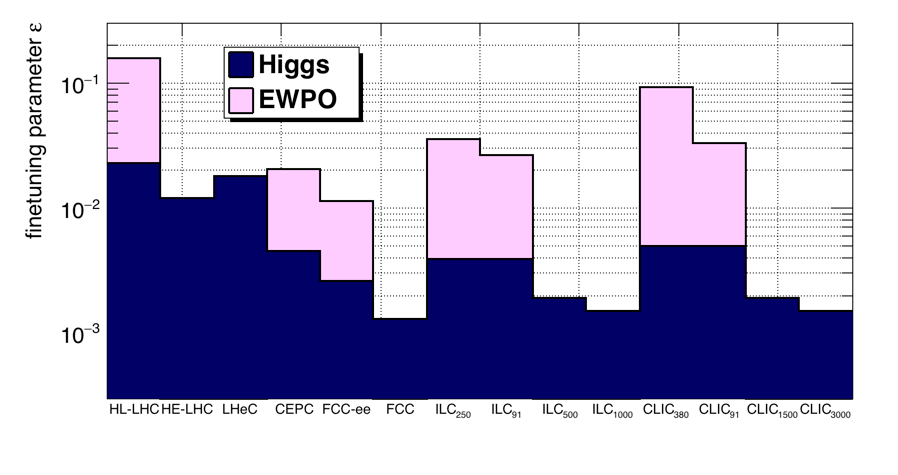
\includegraphics[width=.9\linewidth]{\main/ewksection/img/finetuning}
\caption{\label{fig:h3-finetune}
Finetuning sensitivity as defined in Sec~\ref{sec:ewkintro} based on the Higgs coupling and EWPO precision. In each case the highest precision Higgs measurement is shown based on the EFT analysis: for HL-LHC, HE-LHC and LHeC this is the $ggH$ coupling, and for all others it is the $VVH$ coupling. For the EWPO the value of $S$ is chosen, and multiplied by three to be a measure of $\epsilon$. For the EWPO, only the low-energy stages of the lepton colliders are shown.
}
\end{figure}

In conclusion, the \ew physics programme is pivotal to the understanding of our Universe, relating to important open questions such as the naturalness of our theory, dark matter or the \ew phase transition in the early Universe and the matter-antimatter asymmetry. Many of the proposed accelerators would hugely advance this field of research.

% here are some extra materials that should not be released.
%\newpage
\subsection{Temporary repository for synergy suggestions}

\begin{itemize}
    \item EWK phase transition: LISA
    \item Fine structure constant measurements: AMO
\end{itemize}

\subsection{Temporary repository for cross references to be made with other sections}

\begin{itemize}
    \item need the accelerators to be defined in accelerator part by Lenny and Caterina.
    \item need the hierarchy problem to be discussed in introductory chapter by Gian
    \item reference to BSM section for DM and naturalness
    \item reference to flavor for CP
\end{itemize}

%\bibliography{\main/section1/bib/section}

\subsection{Things that could be put into an appendix or that are useful to keep while finalizing our chapter}
\begin{table}[]
    \centering
    \caption{Number of $Z$ bosons and $W$-pairs for each of the colliders at various $\sqrt{s}$ values. The LEP and SLC numbers reflect the numbers actually produced.
    \label{tab:ewkprogramme}
    \KE{LEP: 4 detectors, each with integrated luminosity of about 200 pb$^{-1}$
SLC: 600,000 measured, 350,000 in last two years.
LEP: numbers for W-pairs include production at threshold and above.}
\BH{CLIC 380, information by email from Philipp Rohloff assumes 50:50 split between +80\% and -80\% polarisation.}}
\begin{tabular}{l r|c c|cr|c|c}
         Collider                          & $\sqrt{s}$    & $\Delta t$ (yr) & $\int\cal{L}$d$t$ (\iab)& Particle & Number & Pol. & default plan \\\hline
         LEP\cite{ALEPH:2005ab}            & $\sim M_Z$    & 7 & $0.8\times 10^{-3}$ & Z-boson & $1.7\times 10^7$ & no & yes \\
         SLD\cite{ALEPH:2005ab}            & $\sim M_Z$    & 6 & ? & Z-boson & $6\times 10^5$ & yes & yes \\ 
         \FCCee\cite{Abada:2019zxq} & $\sim M_Z$ & 4 & $150$ & Z-boson & $3\times 10^{12}$ & no & yes \\
         \CEPC\cite{CEPCStudyGroup:2018ghi} & $\sim M_Z$    & 2  & $16$  & Z-boson &$3\times 10^{11}$ & no & yes\\ 
         \ILC\cite{ILCZ}                    & $\sim M_Z$    & 1-3  & $0.1$ & Z-boson & $4.9\times 10^9$ & yes & no \\
         \CLIC\cite{CLICZ}                  & $\sim M_Z$    & few  & $0.1$ & Z-boson & $5\times 10^9$ & yes & no \\ 
         \ILC\cite{ILCZ}                    & $250$ GeV     & 11  & $2$ & Z-boson & $1.1\times 10^8$ & yes & yes \\
         \CLIC\cite{CLICZ}                  & $380$~GeV     & 8 & $1$ & Z-boson & $5\times 10^6$ & yes & yes \\\hline
         LEP\cite{Schael:2013ita}          & $\gtrsim 2M_W$& 5 & $3\times 10^{-3}$ & W-pairs & $5\times 10^4$ & no & yes \\
         \FCCee\cite{Abada:2019zxq}    & $\sim 2M_W$   & 2 & $12$ & W-pairs & $1\times 10^6$ & no & yes \\
         \CEPC\cite{CEPCStudyGroup:2018ghi} & $\sim 2M_W$   & 1  & $2.6$ & W-pairs & $1.5\times 10^7$ & no &yes\\
         \CEPC\cite{CEPCStudyGroup:2018ghi} & $240$~GeV     & 7 & $5.6$ & W-pairs & $9.5\times 10^7$ & no & yes\\
         \FCCee\cite{Abada:2019zxq}    & $240$~GeV     & 4 & $5$ & W-pairs & $8.5\times 10^7$ & no & yes\\
         \ILC\cite{Fujii:2017vwa}           & $250$~GeV     & 11 & 2 & W-pairs & $3.4\times 10^7$ & yes & yes\\
         \CLIC                              & $380$~GeV     & 8 & 1 & W-pairs& $1.3\times 10^7$ & yes & yes\\
    \end{tabular}
\end{table}

\begin{table}[htbp]
    \centering
    \caption{Higgs coupling measurements from ATLAS~\cite{atlashcomb2}, using between $36.1$ and $79.8$~fb$^{-1}$ for most analyses, and CMS~\cite{cmshcomb2}, using $35.9$~fb$^{-1}$ for all analyses\label{tab:higgsnow}. For the ATLAS $\kappa_t$ result only the allowed values with $\kappa_t>0$ are shown. The \HLLHC projections are also shown based on Ref.~\cite{deBlas:2019rxi}. \BH{Removed table from main text as we now have a nice plot containing the information.}
    \label{higgsnow}
    }
    \begin{tabular}{c|r|r|r}
    \hline
    parameter & ATLAS & CMS & \HLLHC\\\hline\hline
       $\kappa_Z$, $\kappa_V\leq 1$ & $> 0.87$ at 95\% CL & $-0.87 \pm 0.09$& $> 0.987$ at 95\% CL\\
       $\kappa_W$, $\kappa_V\leq 1$ & $> 0.85$ at 95\% CL & $-1.00^{+0.09}_{-0.00}$& $> 0.983$ at 95\% CL\\
       $\kappa_b$  & $0.88 \pm 0.13$ & $0.91^{+0.17}_{-0.16}$ & $\pm 0.026$\\
       $\kappa_t$  & $[0.93,1.24]$ at 68\% CL & $1.02^{+0.19}_{-0.15}$ &$\pm 0.028$\\
       $\kappa_\tau$  & $0.97 \pm 0.13$ & $0.93\pm 0.13$ & $\pm 0.016$\\
       $\kappa_g$  & $1.01^{+0.13}_{-0.11}$ & $1.16^{+0.18}_{-0.13}$ & $\pm 0.022$\\
       $\kappa_\gamma$  & $0.98 \pm 0.07$ & $0.96 \pm 0.09$ & $\pm 0.017$\\
       $\kappa_\mu$  & n.a. & $0.72 ^{+0.50}_{-0.72}$ & $\pm 0.044$\\
$B(H\to \textrm{inv.})$ & $<0.30$ at 95\% CL & $<0.22$ at 95\% CL & $<0.019$ at 95\% CL\\
$B(H\to \textrm{undet.})$ & $<0.22$ at 95\% CL & $<0.38$ at 95\% CL & $<0.041$ at 95\% CL\\
\hline
    \end{tabular}
\end{table}


\begin{figure}[!ht]
\centering
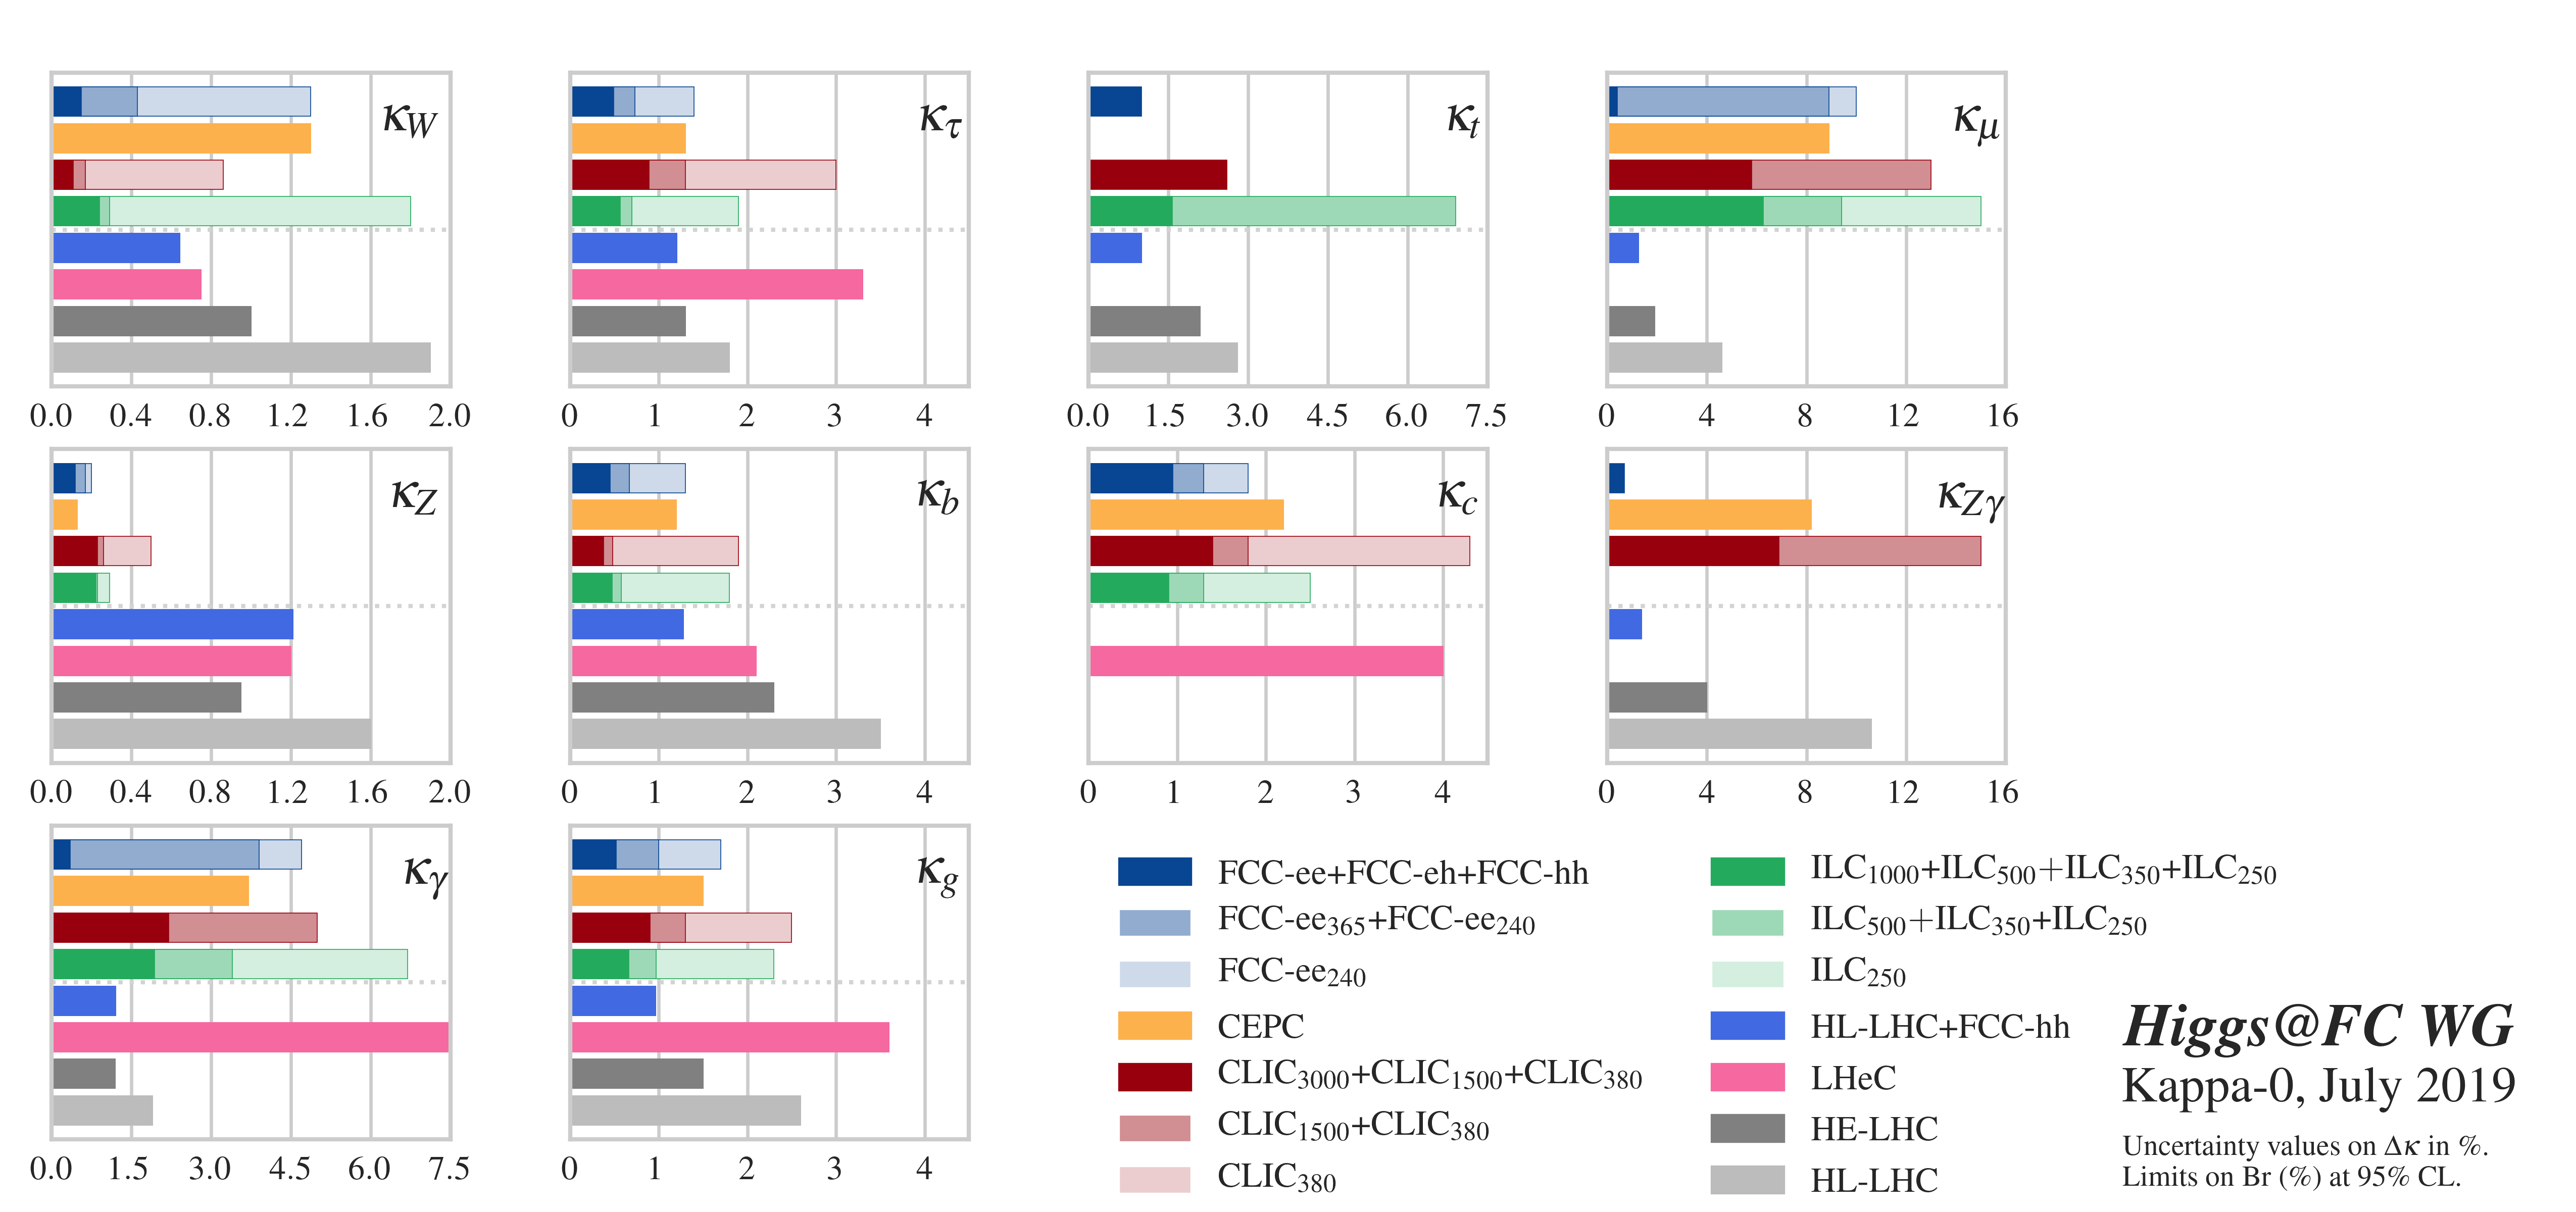
\includegraphics[width=.8\linewidth]{\main/ewksection/img/Kappa0WithNewColumns}
\caption{\label{fig:hkappa0new}
Plot of kappa-0 with \FCChh only and \ILC1000 included.
}
\end{figure}



\end{document}
